%!TEX root=../Thesis_Zepeng.tex
\chapter{Time varying load : the standard approach}\label{chp:4}
\minitoc
%Fatigue failure is a damage accumulation process in which material property deteriorates continuously under
%fatigue loading and the damage depends on the size of
%stress and strain. With the accumulation of fatigue
%damage, some accidents occur for these components. Research shows that a reliable lifetime prediction method is
%particularly important in the design, safety assessments,
%and optimization of engineering components and structures. Thus, it is important to formulate an accurate method
%to evaluate the fatigue damage accumulation and effectively predict the fatigue life of these components.
%The objective of this work is to contribute to the development life model that take into account the presence of complex variations of the stress tensor. We focus on Chaboche damage accumulation law in case of multiaxial high cycle fatigue. Heuristic formulations with different multiaxial fatigue criteria have been proposed. 

\section{The notion of damage in fatigue}


In the case of fatigue, we usually employ the concept of the loading cycle instead of time to evaluate the evolution of damage and to measure the fatigue lifetime. The equations then depend on the load through globally defined quantities over a cycle, such as amplitude, maximum value, mean value.
The growth equation of fatigue damage is therefore taken in the form:
$$\delta D=f(D)\delta N$$
$$\delta N=f_n\delta t$$
where $\delta t$ is a time sampling of the history in a given number of time intervals $\delta t_1,\delta t_2 ... \delta t_i, ...$ and $f_n$ is the mean frequency of those cycles during the considered time step. The issue is thus to identify the function $f(D,S_a,S_m)$ relating the damage growth to the present damage, the load amplitude, the load mean value and so on. We will focus in this chapter on the classical ways of taking into account a possible dependence on $D$.

\subsection{Linear and nonlinear accumulation of damage}
Cumulative effects, whether linear or nonlinear, are of great importance in fatigue. The rule of linear accumulation is in fact a property of any linear or nonlinear differential equation with separable variables. One approach to variable load histories uses the concept of fraction of life(also referred to as cycle ratio) used up by an event. These fractions are added together; when their sum reaches 1.0 or 100 percent we expect failure. This is the most common measure of damage, and is the quantifying measure we present here. 

The Palmgren-Miner linear rule as explained in \cite{lemaitre1990mechanics} is based on the assumption that damage is accumulated additively when it is defined by the associated life ratio $N_i/N_{Fi}$ where $N_i$ is the number of cycles applied under a given load for which the number of cycles to fracture(under periodic conditions) would be $N_{Fi}$. The fracture criterion is:
$$\sum_{i}N_i/N_{F_i}=1.$$
Therefore, in periodic tests, damage evolution is considered to be linear in that:
$$D=N/N_F.$$
For a test at two stress levels, the evolution is as shown schematically in \figref{linear accumulation}. In fact, the linear accumulation rule can be applied even to a damage which evolves nonlinearly. For this it is sufficient that a one-to-one relationship between $D$ and $N/N_F$ exists, or even that the damage evolution curve be a unique function(independent of the applied cycle) of the life ratio $N/N_F$ . 

There are, therefore, two ways of defining a damage incremental law incorporating the linear accumulation rule. It can be linear of the form described below and shown in \figref{linearevolution}:
$$\delta D= \delta N/N_F(...),$$
\begin{figure}[!h]
	\centering
	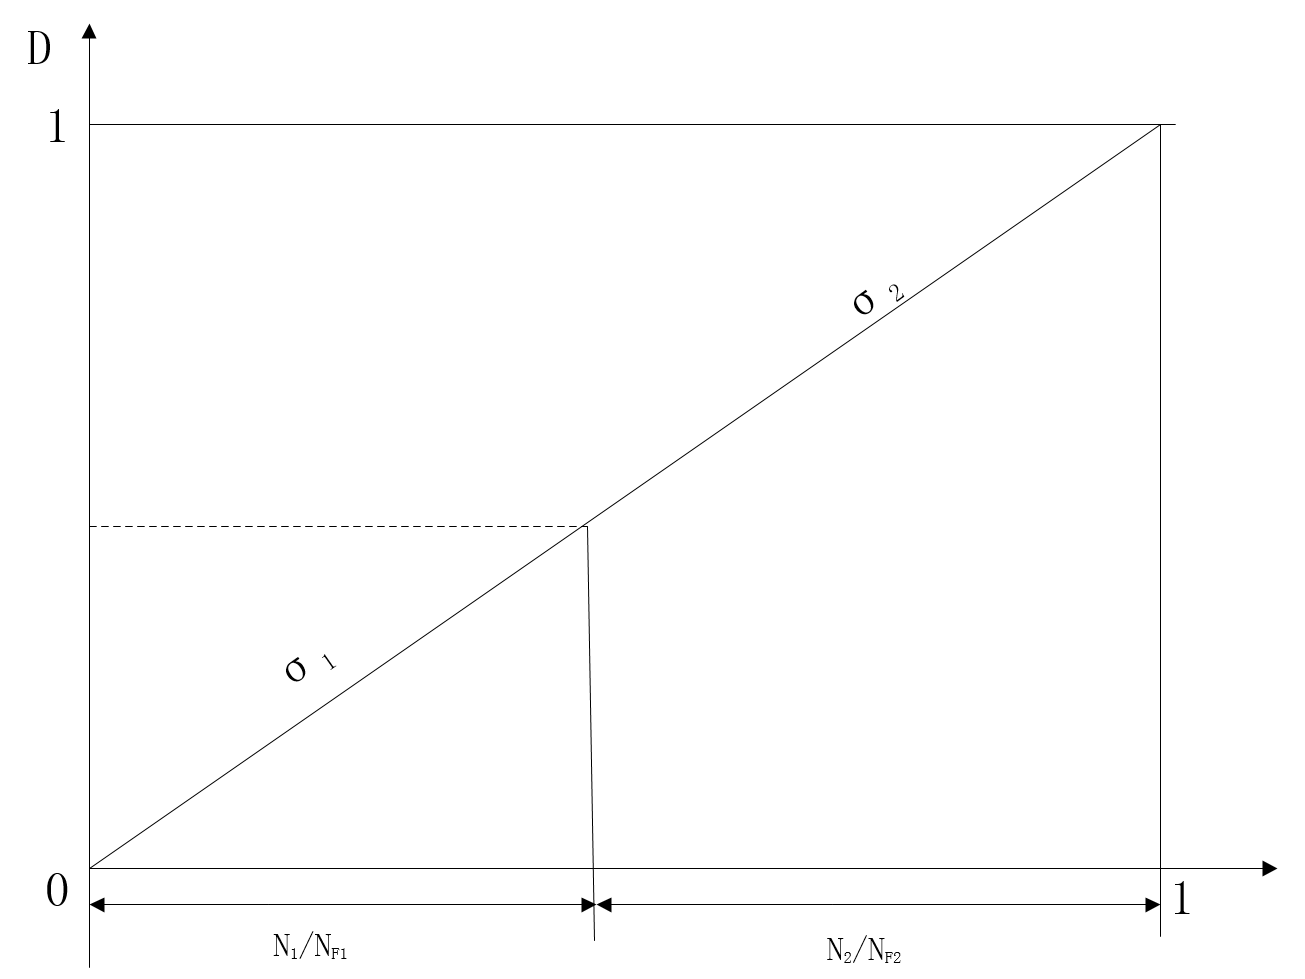
\includegraphics[width=0.8\textwidth]{figures//linearevolution.png} 
	\caption{Linear accumulation of damage with linear evolution}
	\label{linearevolution}
\end{figure}
where $N_F$ is the number of cycles to failure defined by the chosen parametric data.
The damage evolution can be nonlinear such as:
$$\delta D= \frac{(1-D)^{-k}}{k+1}\frac{\delta N}{N_F(...)}.$$
Above, the damage evolution curve as function of life ratio $\delta N/N_F$ is supposed to be independent of the local state of stress (\figref{linear accumulation}).
\begin{figure}[!h]
	\centering
	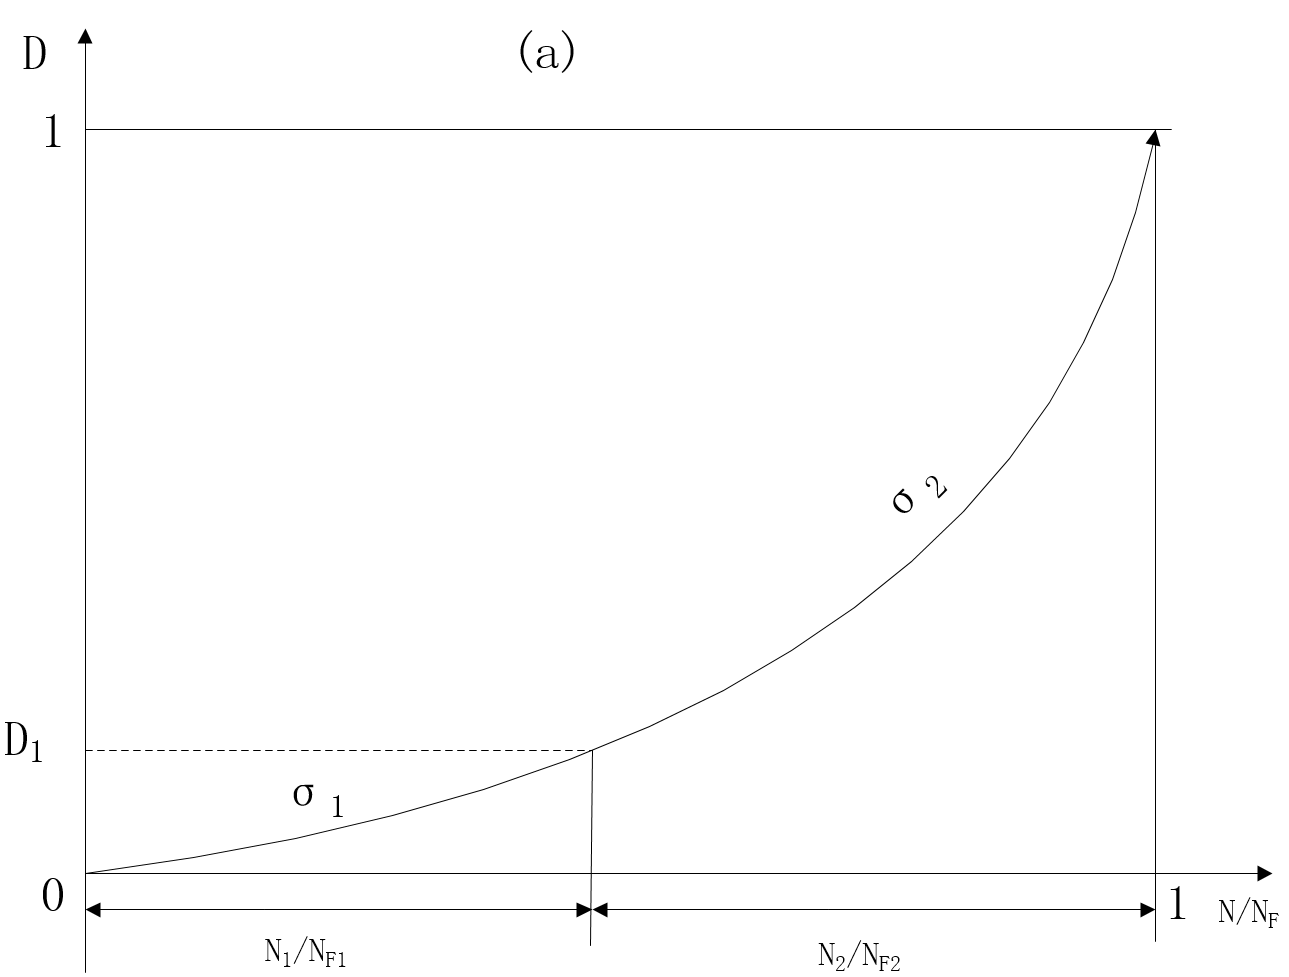
\includegraphics[width=0.8\textwidth]{figures//linearaccumulation.png} 
	\caption{Damage with nonlinear evolution and linear accumulation, where high then low stress loading sequence leads to the same fatigue life.}
	\label{linear accumulation}
\end{figure}
In contrast, if the damage evolution curve,as a function of the life ratio $N/N_F$, depends on the applied loading we have the effect of nonlinear accumulation as shown in \figref{nonlinear accumulation}. 
\begin{figure}[!h]
	\centering
	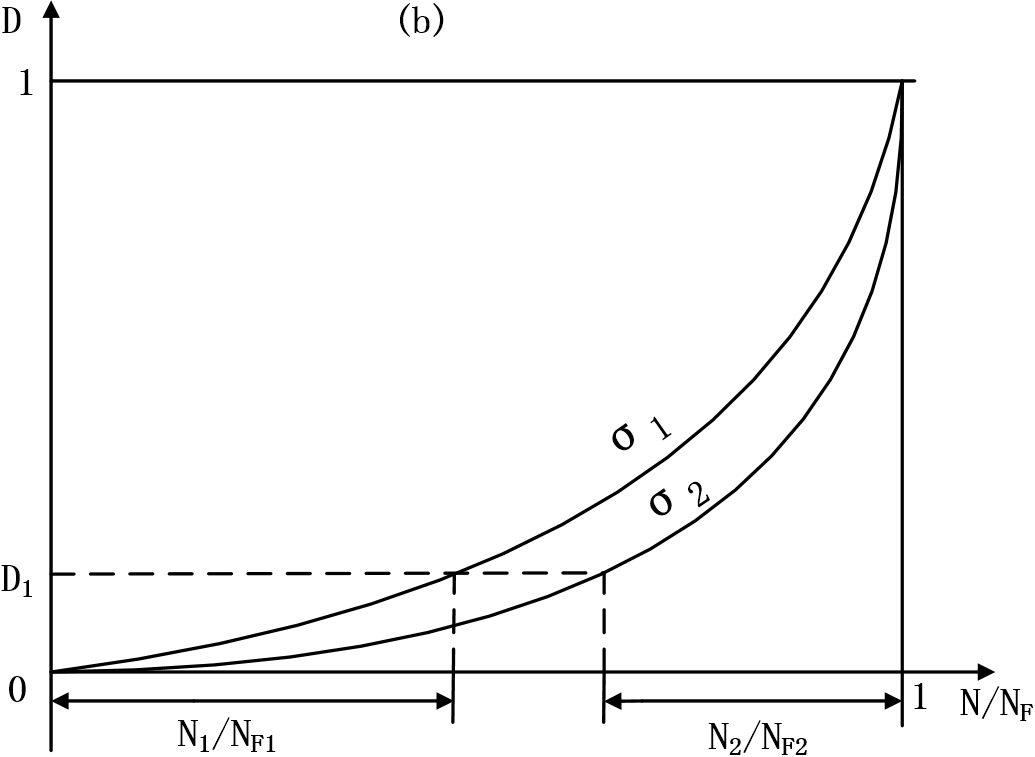
\includegraphics[width=0.8\textwidth]{figures//nonlinearaccumulation.png} 
	\caption{Damage with nonlinear evolution and nonlinear accumulation, where high stress and low stress follow different damage evolution curve. This leads to differences into the summation of fatigue life proportion between different loading sequences.}
	\label{nonlinear accumulation}
\end{figure}
There, $D_1$ represents the state of internal damage at the end of the first level $\sigma_1$. Evolution at the second level $\sigma_2$ continues from the same state, and it is clear that the sum of the life ratio is less than 1. From the point of view of the damage law, this nonlinearity always corresponds to the case where the variables which represent the load $\sigma$ and the damage variable $D$ have coupled evolution.

The Palmgren-Miner linear accumulation law gives good results for loads for which there is little variation in the amplitude and mean value of stress. The assumption of linear damage is open to many objections. For example, sequence and interaction of events may have major influences on life, the rate of damage accumulation may depend on the load amplitude, experimental evidence often indicates that $\sum_{i}N_i/N_{F_i}\neq 1$ for a low-to-high or a high-to-low loading sequence, all effects which are not taken into account in the linear damage assumption.

\newpage
\subsection{Classic Chaboche damage law}

In cyclic loading, one way of writing a damage law which expresses the experimental results is to assume that the damage per cycle is a function of the maximum and the mean values of the stress:
$$\delta D/\delta N=f(\sigma_{Max},\sigma_m).$$
In order to recover, after integration, one of the many forms proposed to represent the Wohler curves, Chaboche (\cite{FFE:FFE1}) proposes to use a law such as:
\begin{equation}
\delta D/\delta N=\frac{\sigma_{Max}-\sigma_l(\sigma_m)}{\sigma_{u}-\sigma_{Max}}\left( \frac{\sigma_{Max}-\sigma_m}{B(\sigma_m)}\right) ^{\gamma}.
\label{generalchaboche}
\end{equation}
with:

$\sigma_l(\sigma_m)=\sigma_m+s_{-1}(1-b\sigma_m)$ :  fatigue limit.

$B(\sigma_m)=B_0(1-b\sigma_m)$ : the mean stress component in the fatigue limit.

$\sigma_u$ : ultimate stress of the material.

The number of cycles to failure is obtained by an obvious integration, with the condition:

$N=0 \to D=0$(initial undamaged state),

$N=N_F \to D=1$(macro-crack initiation).

By integration Eq.\eqref{generalchaboche} from $D=0$ to $D=1$ we therefore get:
\begin{equation}N_F=\frac{\sigma_{u}-\sigma_{Max}}{\sigma_{Max}-\sigma_l(\sigma_m)}\left(\frac{\sigma_{Max}-\sigma_m}{B(\sigma_m)}\right)^{-\gamma}.
\label{NF}
\end{equation}

Eq.\eqref{generalchaboche} then writes:
$$\delta D=\dfrac{\delta N}{N_F(\sigma_{Max},\sigma_{u})}.$$

The constants are determined from conventional data:$\sigma_u$ is usually known, $s_{-1},b$ fit the results on the fatigue limits with relation $\sigma_l(\sigma_m)=\sigma_m+s_{-1}(1-b\sigma_m)$. Exponent $\gamma$ is obtained from the S-N curve for reversed conditions, by plotting $\sigma_{Max}$ as function of $N_F(\sigma_{Max}-\sigma_l(\sigma_m))/(\sigma_{u}-\sigma_{Max})$, as deduced from Eq.\eqref{NF}. Coefficient $B(\sigma_m)$ is obtained from one point of the S-N curve.

\vspace{6pt}
\textbf{Uniaxial case}
\vspace{6pt}

The equation studied below allows us to describe the effects of nonlinear accumulation in the case of non-periodic cyclic loads (\cite{FFE:FFE1}). A simple way to introduce such effects in the damage growth equation consists in rendering the load and damage variables non-separable. For example, we may take:
$$\delta D=D^{\alpha(\sigma_{Max},\sigma_m)}\left(\frac{\sigma_{Max}-\sigma_m}{B(\sigma_m)}\right)^\gamma\delta N$$
The exponent $\alpha$ depends on the loading $(\sigma_{Max},\sigma_m)$, which results in non-separability. A reference choice is

\vspace{6pt}
$$\alpha(\sigma_{Max},\sigma_m)=1-a\left\langle\dfrac{\sigma_{Max}-\sigma_l(\sigma_m)}{\sigma_u-\sigma_{Max}}\right\rangle$$
\vspace{6pt}

The exponent $\alpha$ represents the effect of the internal variables(for example the hardening state of the material), which depends on the loading $(\sigma_{Max},\sigma_m)$, resulting in non-separability. It induces allows a non-linear damage cumulative rule as it is experimentally observed. Above, $a$ and $\gamma$ are material parameters. The coefficients $\gamma$ is determined from experimental Woehler's curves. 

The concept of effective stress applied to fatigue provides an indirect measure. The measured evolutions are extremely nonlinear. With this concept, damage can really be measured only in the last part of the life-time, when microscopic initiations have already occurred(this is the phase of micro-propagation of defects). And these damage evolutions are extremely nonlinear. To reproduce this phenomenological aspect it is sufficient to make a change of variable by replacing $D$ in the previous equation by a different measure of damage described by:
$$1-(1-D)^{\gamma+1}.$$
The differential law can be written as:
\begin{equation}\delta D=[1-(1-D)^{\gamma+1}]^{\alpha(\sigma_{Max},\sigma_m)}\big[\frac{\sigma_{Max}-\sigma_m}{M(\sigma_m)(1-D)}\big]^\gamma\delta N
\label{diff}
\end{equation}

This form is more complex, but its properties are identical to the properties of the previous equation, except for the current value of damage. Now we integrate it to see how damage $D$ evolves with cycle numbers $N$ and the influence of different parameters. By differential calculus, we get from Eq.\eqref{diff}:
\begin{equation}\delta [1-(1-D)^{\gamma+1}]^{1-\alpha}=(1-\alpha)(\gamma+1)\big[\frac{\sigma_{Max}-\sigma_m}{M(\sigma_m)}\big]^\gamma\delta N.
\label{easyintegration}
\end{equation}


The number of cycles to failure, obtained by integrating $D$ from 0 to 1 is thus:
\begin{equation}N_F=\frac{1}{(\gamma+1)(1-\alpha)}\left(\frac{\sigma_{Max}-\sigma_m}{M(\sigma_m)}\right)^{-\gamma}
\label{eqnf}
\end{equation}
and we find by comparing with Eq.\eqref{NF} that $M(\sigma_m)=B(\sigma_m)(\gamma+1)^{1/\gamma}$. This form Eq.\eqref{eqnf} can be used in experimental Woehler's curve in order to identify the coefficient $a$ and $\gamma$. In differential form,  from Eq.\eqref{easyintegration} and Eq.\eqref{eqnf}, we get equivalently
\begin{equation}\delta [1-(1-D)^{\gamma+1}]^{1-\alpha}=\frac{\delta N}{N_F}
\label{diffform}
\end{equation}
When we integrate Eq.\eqref{easyintegration} from $0$ to $D$ at constant loading conditions, the damage, expressed as a function of $N/N_F$ is:
\begin{equation}D=1-\left[ 1-\left( \frac{N}{N_F}\right) ^{\frac{1}{1-\alpha}}\right] ^{\frac{1}{\gamma+1}}.
\end{equation}
This expression is in good agreement with experimental results (\cite{lemaitre1990mechanics}). 

\vspace{6pt}
\textbf{Multiaxial case}
\vspace{6pt}

The applied stress and strain tensors are often multiaxial and present a complex path during a loading cycle. In the case of multiaxial loading fatigue, the Chaboche model is represented by the following equation:
\begin{equation}\delta D = \left( 1 -(1-D)^{\gamma+1}\right)^\alpha \left(\frac{\widetilde{A}_{\uppercase\expandafter{\romannumeral2}}}{M(\sigma_H)}\right)^\gamma \delta N
\label{chabochemulti}
\end{equation} 
where the amplitude $\sigma_{Max}-\sigma_l(\sigma_m)$ is replaced by the deviatoric norm $A_{\uppercase\expandafter{\romannumeral2}}$ and the average stress is replaced by the hydrostatic pressure. We should note that for an isotropic damage theory, we will have from Eq.\eqref{easyintegration}
$$\widetilde{A}_{\uppercase\expandafter{\romannumeral2}}=A_{\uppercase\expandafter{\romannumeral2}}/(1-D)$$

\begin{equation}\alpha = 1 - a\left\langle \frac{A_{\uppercase\expandafter{\romannumeral2}} - A_{\uppercase\expandafter{\romannumeral2}}^\ast(\sigma_H)}{ \sigma_{u} - \sigma_{eqMax}}\right\rangle.\end{equation}

Again, $\alpha$ represents the influence of internal variables,characterizes the non-linearity of the damage evolution, allows to take into account the mean stress effect and describes the damage occurrence of the material: as long as $\alpha < 1$, there is damage creation. The coefficient $a$ gives the amount of fragility which is induced by a given occurrence of fatigue limit violation.

In this formula, $A_{\uppercase\expandafter{\romannumeral2}}$ is the amplitude of octahedral shear stress given by:

\begin{equation}A_{\uppercase\expandafter{\romannumeral2}}=\frac{1}{2}\max\limits_{t}\sqrt{\frac{1}{2}\uline{\uline{\Delta s}}:\uline{\uline{\Delta s}}}=\sqrt{J_2}_a=\frac{1}{2}\Delta\sigma_{eqmax},\end{equation}

The quantity $A_{\uppercase\expandafter{\romannumeral2}}^\ast(\sigma_H)$ represents the infinite life fatigue limit. For example,the Sines fatigue limit criterion is formulated by the following equation:
\begin{equation} A_{\uppercase\expandafter{\romannumeral2}}^\ast(\sigma_H)=s_{-1}(1-3b\sigma_H).\end{equation}

Above, $s_{-1}$ and $\sigma_{u}$ are respectively the fatigue limit at zero mean stress and the ultimate tensile stress. For steel, we usually have $s_{-1}\approx 0.48\sigma_{u}$.

The function $M(\sigma_H)$ in Eq.\eqref{chabochemulti} quantifies the mean stress effect through Low Cycle Fatigue(LCF) loading range:
$$M(\sigma_H)=s_{-1}\left(1-3\frac{\sigma_H}{\sigma_u}\right).$$

We can get the $D-N$ curve in \figref{DN} by integrating Eq.\eqref{chabochemulti}. This is in the case of constant loading conditions because we regard $\alpha$ and $\gamma$ as invariable parameters.
\begin{equation}N =\frac{( 1 -(1-D)^{\gamma+1})^{1-\alpha}}{(1+\gamma)(1-\alpha)}\left[\frac{A_{\uppercase\expandafter{\romannumeral2}}}{M(\sigma_H)}\right]^{-\gamma} 
\label{D-N}
\end{equation} 

\begin{figure}[!h]
	\centering
	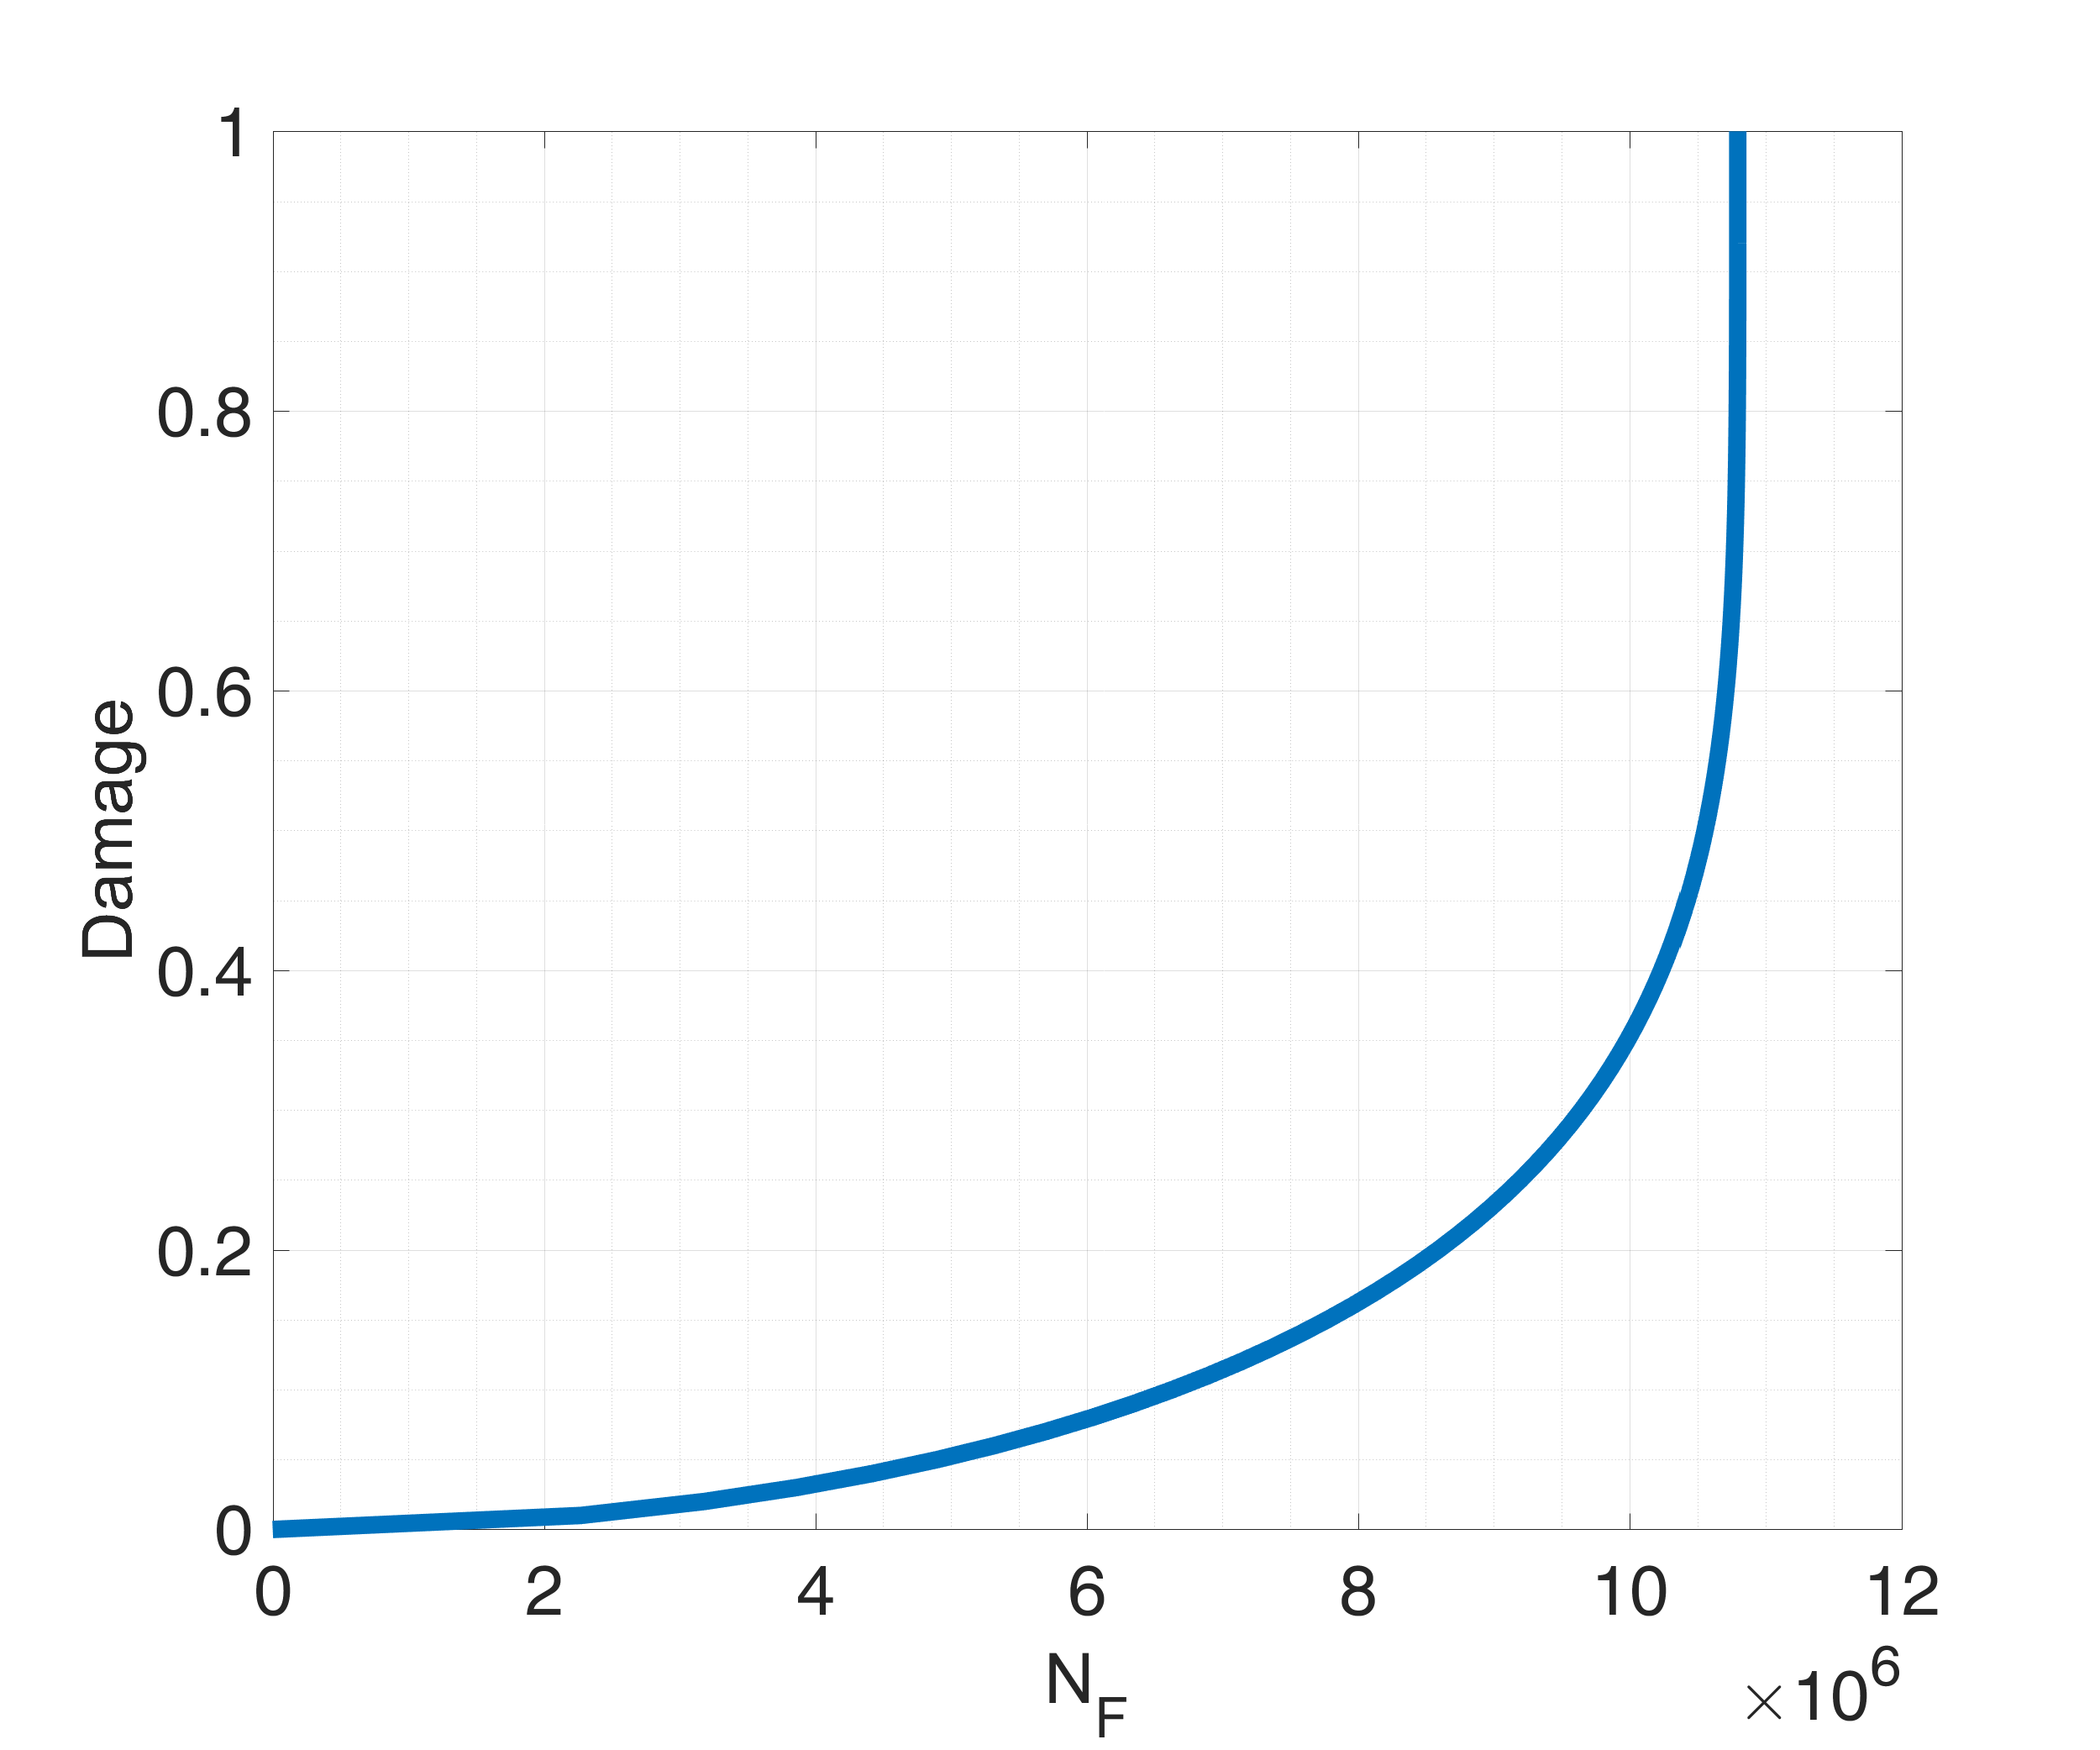
\includegraphics[width=0.8\textwidth]{figures//D-N.png} 
	\caption{Damage accumulation in terms of N in constant loading condition, with D and N are related by the evolution equation \eqref{D-N}}
	\label{DN}
\end{figure}

The number of cycles to failure, obtained at $D=1$, is: 
\begin{equation}N_F = \frac{1}{(\gamma+1)(1-\alpha)}\left[\frac{A_{\uppercase\expandafter{\romannumeral2}}}{M(\sigma_H)}\right]^{-\gamma}
\label{chaboche}
\end{equation} 

In Eq.\eqref{chaboche}, $\gamma$, $b$ and $a$ are material parameters determined from fatigue tests.

In the case of multiaxial fatigue loading, an infinite life is obtained if the stress amplitude $A_{\uppercase\expandafter{\romannumeral2}}$ respects:

\begin{equation}A_{\uppercase\expandafter{\romannumeral2}}\leqslant A_{\uppercase\expandafter{\romannumeral2}}^\ast(\sigma_H)=s_{-1}(1-3b\sigma_H).\end{equation}

In terms of Sines criterion which Chaboche uses, it writes:
\begin{equation}\sqrt{J_2}_a+3bs_{-1}\sigma_H-s_{-1}\leqslant 0.
\label{sines}
\end{equation}

Finally, $\sigma_H$ is the mean hydrostatic stress defined by:
\begin{equation}\sigma_H=\frac{1}{6}[\max tr(\uline{\uline{\sigma}}(n))+\min tr(\uline{\uline{\sigma}}(n))],\end{equation}


In terms of number of cycles at given load, the damage is expressed as in uniaxial case:
\begin{equation}D=1-\left[ 1-\left( \frac{N}{N_F}\right) ^{\frac{1}{1-\alpha}}\right] ^{\frac{1}{\gamma+1}}.
\label{damage}
\end{equation}

\begin{figure}[!h]
	\centering
	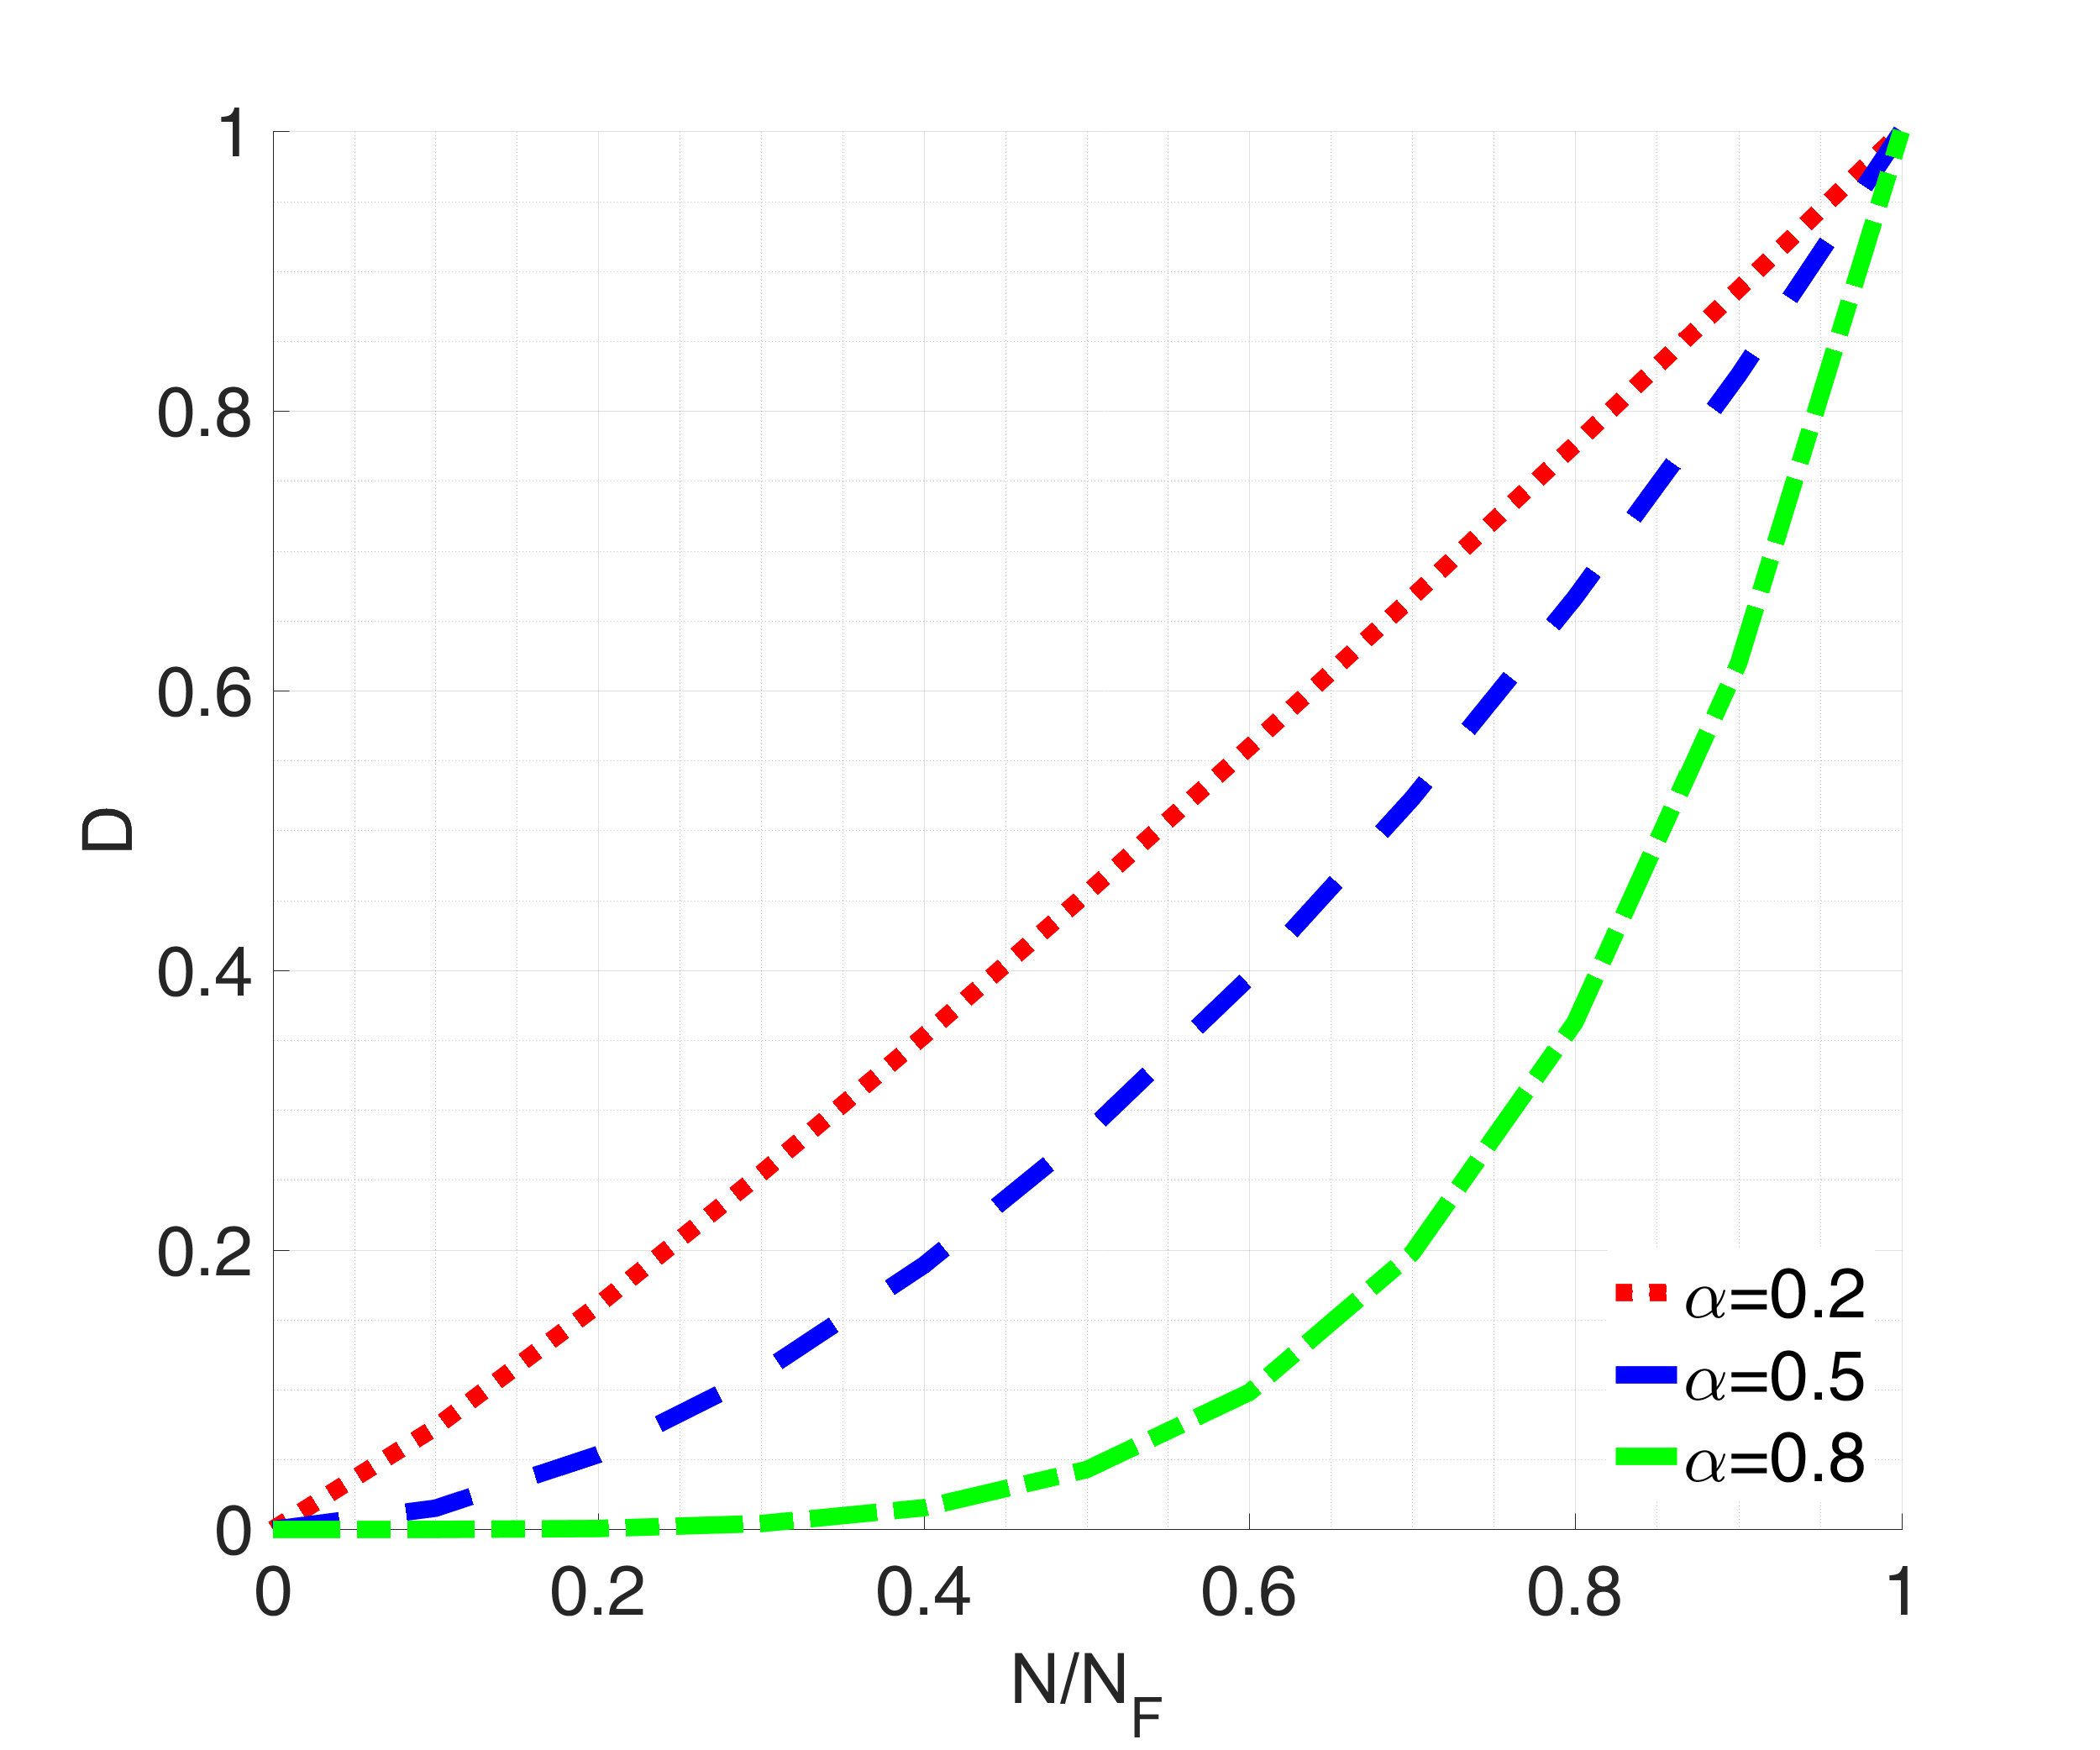
\includegraphics[width=\textwidth]{figures//Dratio1.png}
	\vspace{-12pt}
	\caption{Influence of function $\alpha$ in fatigue damage versus fatigue life ratio ($\gamma=0.1$)}
	\label{Alpha}
\end{figure}
These theories account for the nonlinear nature of fatigue damage accumulation by using nonlinear relations such as Eq.\eqref{damage} where the power $\alpha$ depends on the load level(see \figref{Alpha}). The same equation with frozen $\alpha$ leads to linear damage accumulation.


\begin{figure}[!h]
	\centering
	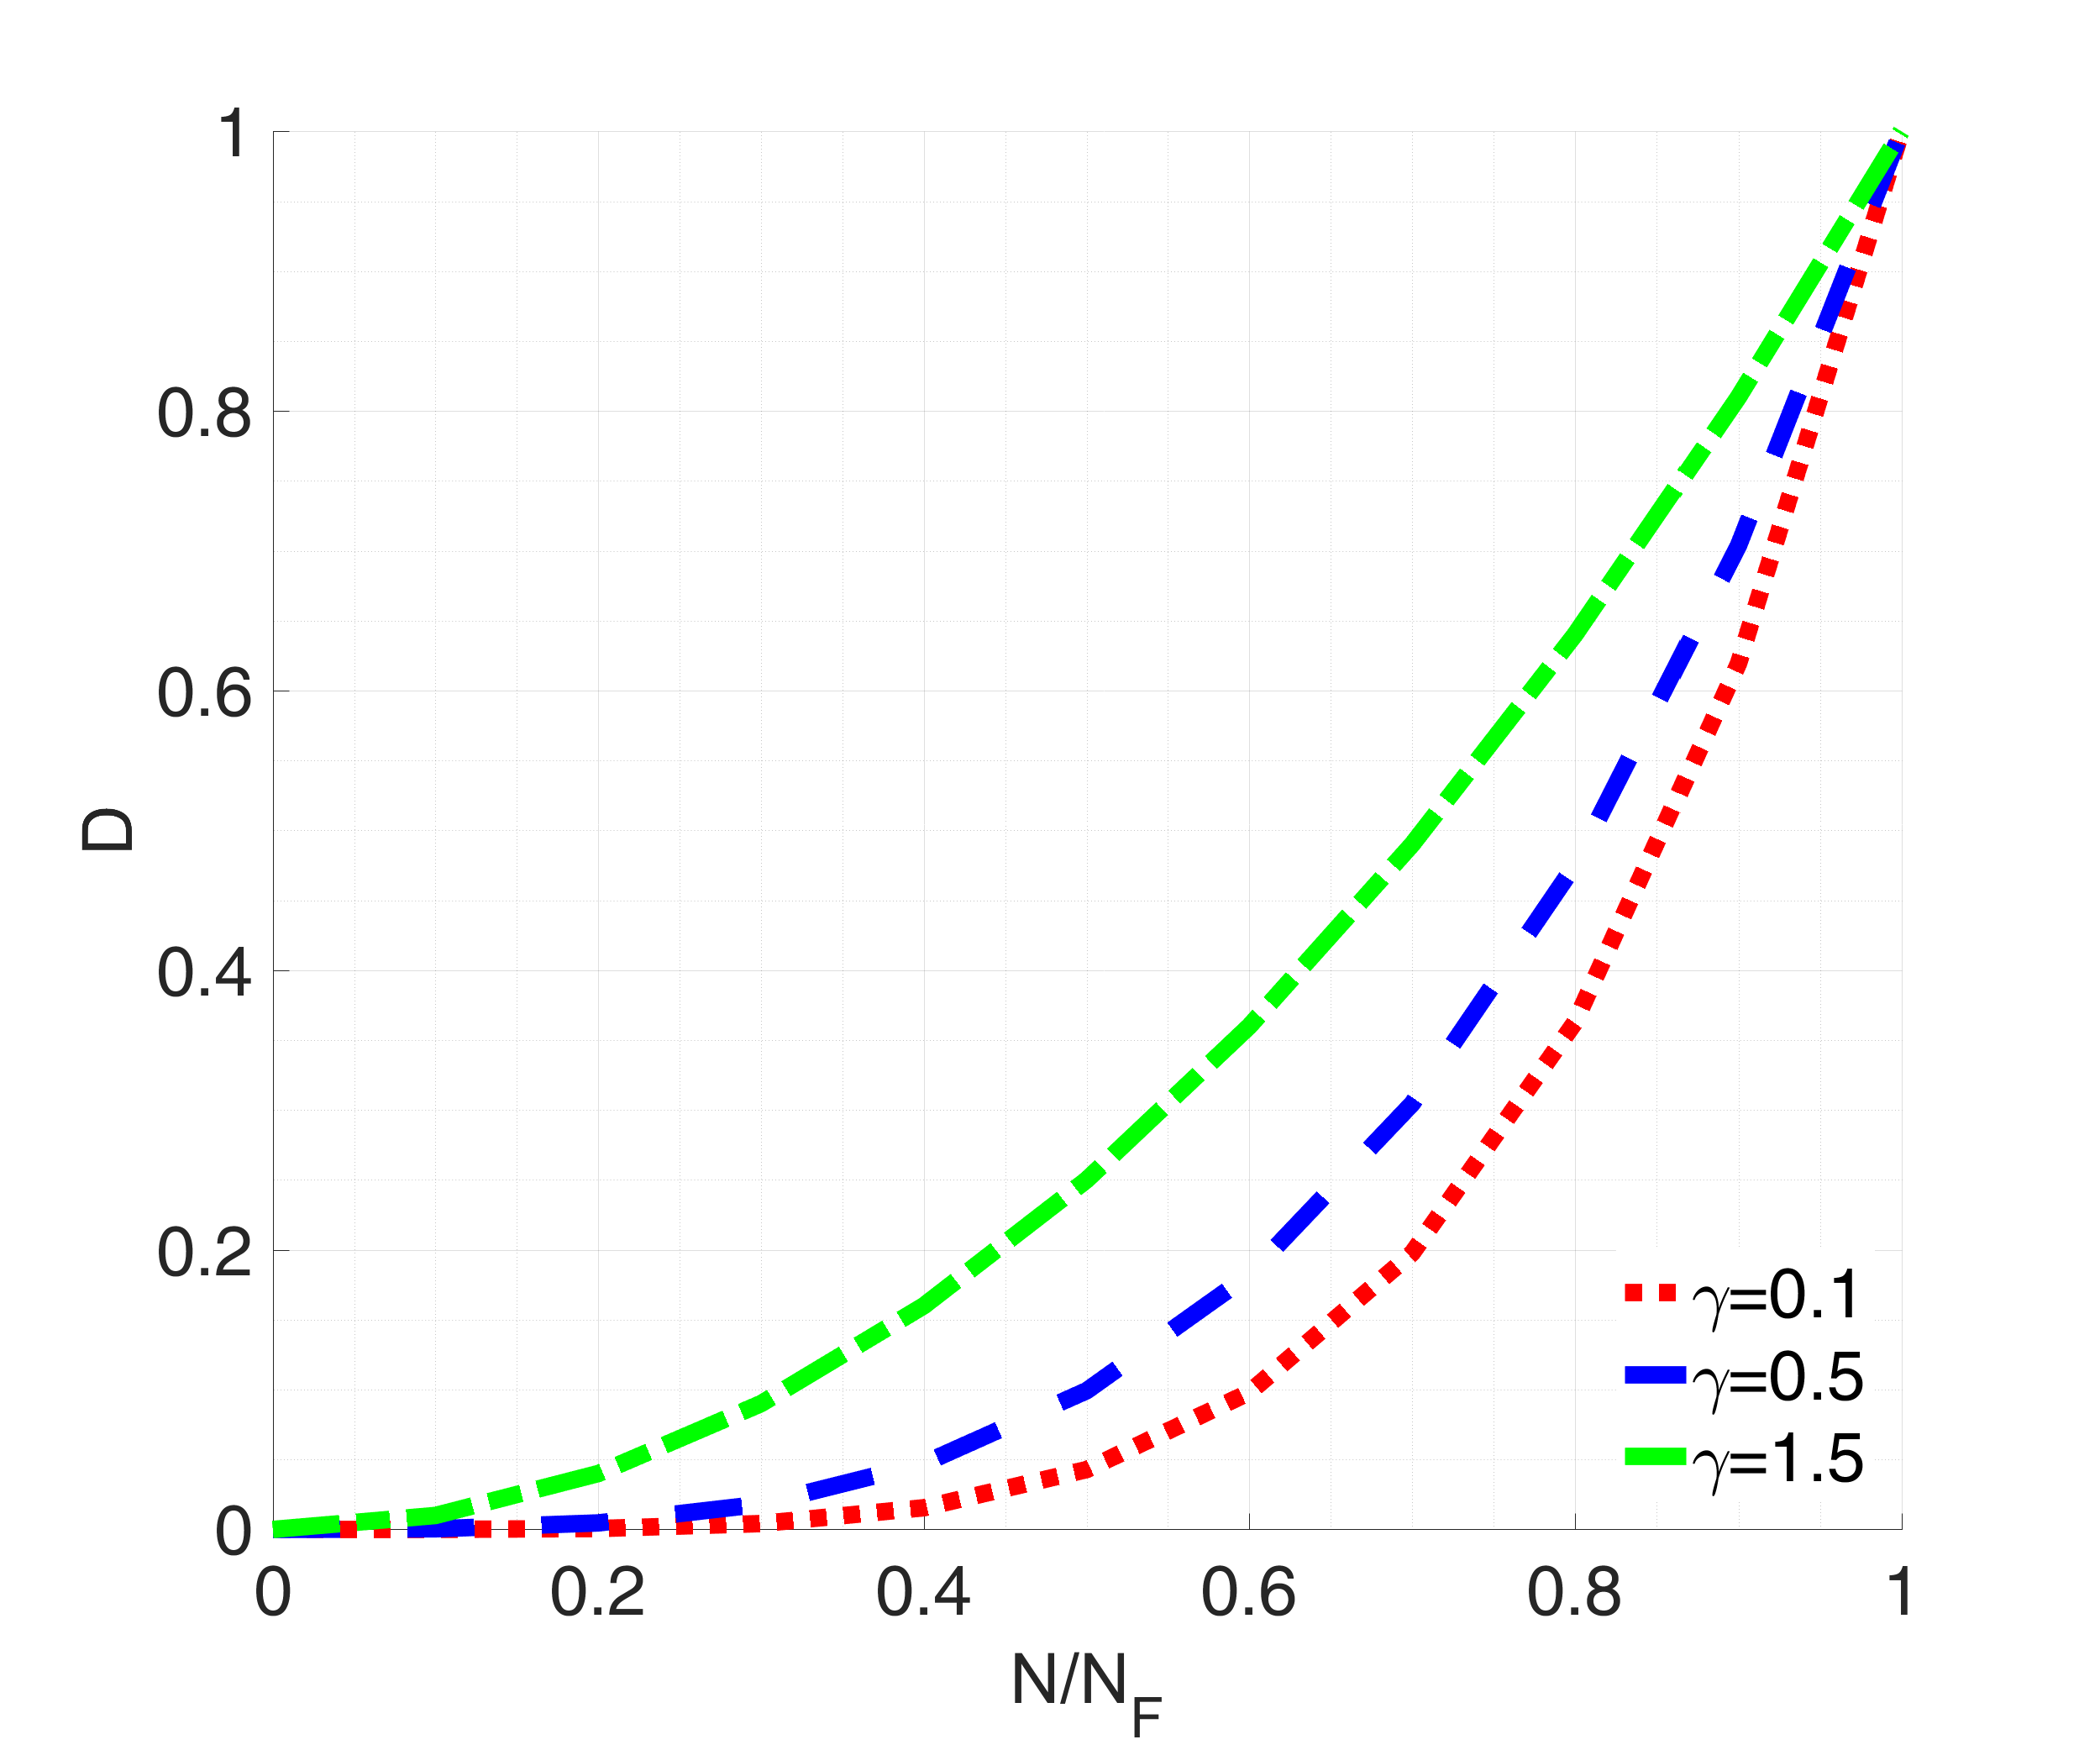
\includegraphics[width=\textwidth]{figures//Dratio2.png}
	\vspace{-12pt}
	\caption{Influence of function $\gamma$ in a plot of  damage versus fatigue life ratio with $\alpha=0.8$}
\end{figure}

\clearpage
\section{Verification method of Chaboche law}

To facilitate our verification of the law we use two-stress level loading, the specimen is firstly loaded at stress $\sigma_1$ for $N_1$ cycles and then at stress $\sigma_2$ for $N_2$ cycles until failure. We can then observe if the experimental results are satisfactory.\\
After $N_1$ cycles, we have from Eq.\eqref{damage}, a damage $D_1$ given by:
\begin{equation}
[1-(1-D_1)^{\gamma+1}]^{1-\alpha_1}=\frac{N_1}{N_{F1}}.
\label{eq.23a}
\end{equation}
By integrating Eq.\eqref{diffform} from $D=D_1$ to $D=1$, we get:
\begin{equation}
1-[1-(1-D_1)^{\gamma+1}]^{1-\alpha_2}=\frac{N_2}{N_{F2}},
\end{equation}
which yields:
\begin{equation}1-\frac{N_2}{N_{F2}}=1-[1-(1-D_1)^{\gamma+1}]^{1-\alpha_2}.
\label{eq.23b}
\end{equation}
From Eq.\eqref{eq.23a} and Eq.\eqref{eq.23b}, after elimination of $[1-(1-D_1)^{\gamma+1}]$ we get:
\begin{equation} \frac{N_2}{N_{F2}}=1-(\frac{N_1}{N_{F1}})^\frac{1-\alpha_2}{1-\alpha_1}=1-(\frac{N_1}{N_{F1}})^\eta\end{equation}
with
\begin{equation}
		\begin{split}
			\eta&=\frac{1-\alpha_2}{1-\alpha_1}
			\\&=\frac{A_{\uppercase\expandafter{\romannumeral2 2}} - A_{\uppercase\expandafter{\romannumeral2}}^\ast(P_{m2})}{A_{\uppercase\expandafter{\romannumeral2 1}} - A_{\uppercase\expandafter{\romannumeral2}}^\ast(P_{m1})}\frac{ \sigma_{u} - \sigma_{eqMax1}}{ \sigma_{u} - \sigma_{eqMax2}}
			\\&=\frac{\sqrt{J_{2,a_2}} - s_{-1}(1-3bP_{m_2})}{\sqrt{J_{2,a_1}} - s_{-1}(1-3bP_{m_1})}\frac{ \sigma_{u} - \max(2\sqrt{J_{2,a_1}})}{  \sigma_{u} - \max(2\sqrt{J_{2,a_2}})}.
	\end{split}
\label{eq.etachaboche}
\end{equation}

In the case of high-low loading sequence($\sigma_1>\sigma_2 \; thus \; \alpha_1<\alpha_2$):

$$\eta=\frac{1-\alpha_2}{1-\alpha_1}<1\Rightarrow \frac{N_2}{N_{F2}}=1-(\frac{N_1}{N_{F1}})^\eta<1-\frac{N_1}{N_{F1}},$$

in other words, we have 
$$\frac{N_1}{N_{F1}}+\frac{N_2}{N_{F2}}<1.$$

The cumulative damage under high-low loading sequence, as we deduced, has the addition of partial lives less than 1. 

Similarly, the cumulative damage under low-high loading sequence has has a beneficial effect: 
$$\frac{N_1}{N_{F1}}+\frac{N_2}{N_{F2}}>1.$$

For constant two-level stress loading, $\alpha_1=\alpha_2$, the Chaboche law returns to the miner's rule where we have:
$$\frac{N_1}{N_{F1}}+\frac{N_2}{N_{F2}}=1.$$
\section{Chaboche law containing different criteria}
\subsection{Chaboche law with Crossland criterion}

In the previous model we used Sines fatigue criterion constructing the damage criterion exponent $\alpha$. Now we want to test Chaboche law with different criteria and compare the numerical results. Since $\alpha$ represents the internal variables and contains the fatigue criterion, we first change $\alpha$ to satisfy Crossland Criterion:

\begin{equation}\alpha = 1 - a\left\langle \frac{\max\limits_{n}\sqrt{J_2}_a(n)+a_c{P_{max}(n)}-b_c}{ \sigma_{u} - 2\max\sqrt{J_2}_a}\right\rangle,\end{equation}

with
\begin{equation}
a_c=\frac{(t_{-1}-\frac{f_{-1}}{\sqrt{3}})}{\frac{f_{-1}}{3}}, \quad 
b_c=t_{-1}.
\end{equation}

Therefore, the coefficient $\eta$ characterizing the high low sequential loading will now be given by
\begin{equation}\eta_c=\frac{1-\alpha_2}{1-\alpha_1}=
\frac{\sqrt{J_{2,a_2}}+a_cP_{M_2}-b_c}{\sqrt{J_{2,a_1}}+a_cP_{M_1}-b_c}\frac{ \sigma_{u} - \max(2\sqrt{J_{2,a_1}})}{  \sigma_{u} - \max(2\sqrt{J_{2,a_2}})}.
\end{equation}

In Eq.\eqref{chabochemulti} and \eqref{D-N}, the amplitude of octahedral shear stress $A_{\uppercase\expandafter{\romannumeral2}}$ remain unchanged.

\subsection{Chaboche law with Dang Van criterion}

We can also change $\alpha$ to express it through Dang Van Criterion, leading to:

\begin{equation}\alpha = 1 - a\left\langle \frac{\max\limits_{n}\left\{\tau{(n)}+a_DP{(n)}\right\}-b_D}{ \sigma_{u} - 2\max\sqrt{J_2}_a}\right\rangle.\end{equation}

with
\begin{equation}
\tau(n)=\frac{1}{2}(\hat{\sigma}_{\Rmnum{1}}(n)-\hat{\sigma}_{\Rmnum{3}}(n))
\end{equation}
$$a_D=\frac{3t_{-1}}{f_{-1}}-\frac{3}{2}, b_D=t_{-1}.$$
In this case, the coefficient $\eta$ of high low sequential loading becomes
\begin{equation}\eta_D=\frac{1-\alpha_2}{1-\alpha_1}=
\frac{\max\limits_{t}\left\{\tau_2{(n)}+a_DP_2{(n)}\right\}-b_D}{\max\limits_{t}\left\{\tau_1{(n)}+a_DP_1{(n)}\right\}-b_D}\frac{ \sigma_{u} - \max(2\sqrt{J_{2a_1}})}{  \sigma_{u} - \max(2\sqrt{J_{2a_2}})}
\end{equation}
In Eq.\eqref{chabochemulti} and \eqref{D-N}, we change $A_{\uppercase\expandafter{\romannumeral2}}$ to $\max\tau(n)$:
\begin{equation}N_F = \frac{1}{(\gamma+1)(1-\alpha)}\left[\frac{\max\tau(n)}{M(\sigma_H)}\right]^{-\gamma}
\label{dvchaboche}
\end{equation} 

\section{Numerical testing on different loading patterns}
The fatigue limit with different criteria are distinctive. We compare different criteria in a $A_{\uppercase\expandafter{\romannumeral2}}-N_F$ figure as predicted in Eq.\eqref{chaboche}. Here
$\gamma$, $b$ and $a$ are material parameters determined from fatigue tests.

In this case we have 
$$N_F = \frac{1}{(\gamma+1)(1-\alpha)}\left[\frac{A_{\uppercase\expandafter{\romannumeral2}}}{M(\sigma_H)}\right]^{-\gamma},$$

$$M(\sigma_H)=s_{-1}\left(1-3\sigma_H/\sigma_u\right).$$

For Sines and Crossland criteria:

$$A_{\uppercase\expandafter{\romannumeral2}}=\sqrt{J_2}_a=\frac{1}{2}\max\limits_{t}\sqrt{\frac{1}{2}(\Delta s_{11}^2+\Delta s_{22}^2+\Delta s_{33}^2+2\Delta s_{12}^2+2\Delta s_{13}^2+2\Delta s_{23}^2)}.$$

For Dang Van criterion:
$$A_{\uppercase\expandafter{\romannumeral2}}= \max\tau(n).$$ 


\subsection{Test on pure rotation}

From the fatigue zone we select $r=0.1$ as the radius to study. We select here:

$s_{-1}=f_{-1}=0.8MPa$,

$\sigma_{u}=1.67MPa$ 

$\gamma=6$


$A_{\uppercase\expandafter{\romannumeral2}}-N_F$ figure is shown in \figref{JNrotation}. 
\begin{figure}[!h]
	\centering
	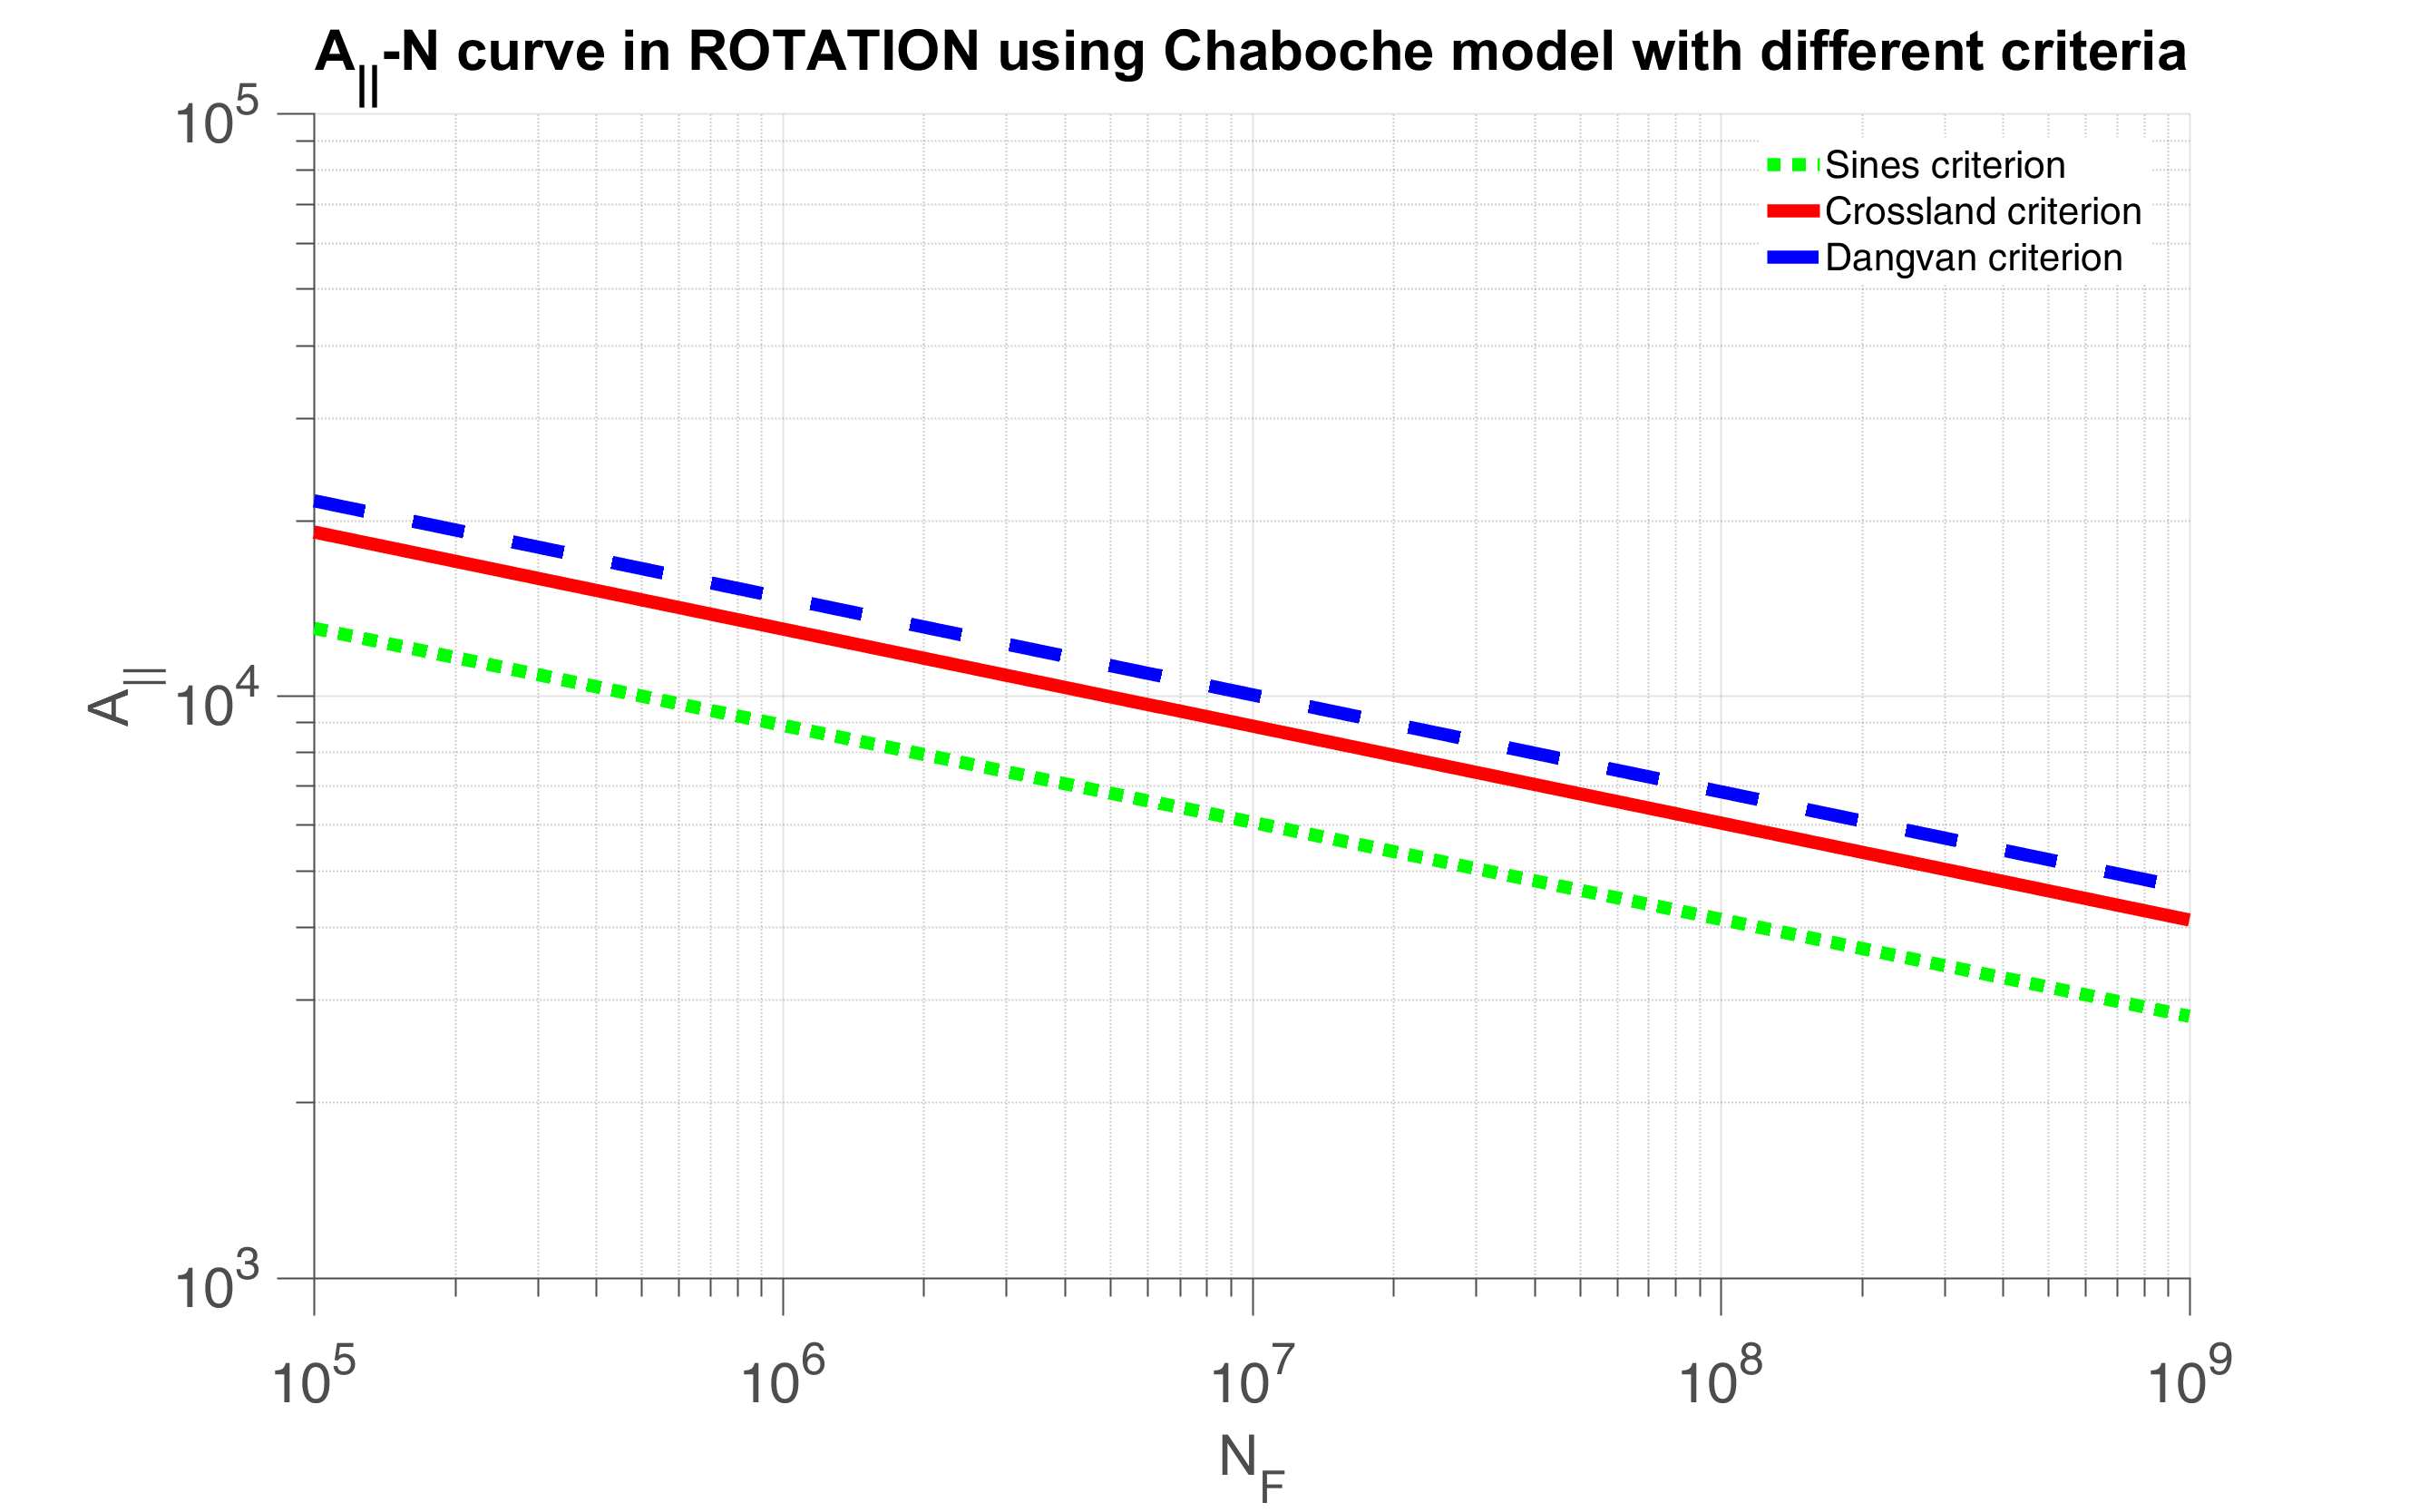
\includegraphics[width=\textwidth]{figures//JNrotation.png} 
	\caption{$A_{\uppercase\expandafter{\romannumeral2}}-N_F$ curve in rotation at r=0.1}
	\label{JNrotation}
\end{figure}

In pure rotation, we assume the first and second rotating speed are respectively $w_1=20rpm$ and $w_2=15rpm$.  

\vspace{6pt}
$A_{\uppercase\expandafter{\romannumeral2}1}=\sqrt{J_{2,a_1}}=7.7606E5 Pa$

\vspace{6pt}
$A_{\uppercase\expandafter{\romannumeral2}2}=\sqrt{J_{2,a_2}}=4.3653E5 Pa$

\vspace{6pt}
$P_{m_1}=8.8342E5 Pa$

\vspace{6pt}
$P_{m_2}=4.9693E5 Pa$

Substituting the above to Eq.\eqref{eq.etachaboche}, we can get $\eta$ in High-Low sequence and in Low-High sequence as shown in Table.\ref{tab.etarotation}:

\begin{table}[!h]
	\centering
	\begin{tabular}{llll}
		\hline
		$\eta$ value   & Sines  & Crossland & Dang Van \\ \hline
		High-low & 0.0721 & 0.0219    & 0.0121   \\
		Low-high & 13.8654 & 45.6118   & 82.5689  \\ \hline
	\end{tabular}
	\caption{$\alpha$ induced sequence effect parameter $\eta$ value with different criteria in pure rotation}
	\label{tab.etarotation}
\end{table}

The predicted results are shown in \figref{2stressR}.

\begin{figure}[!h]
	\centering
	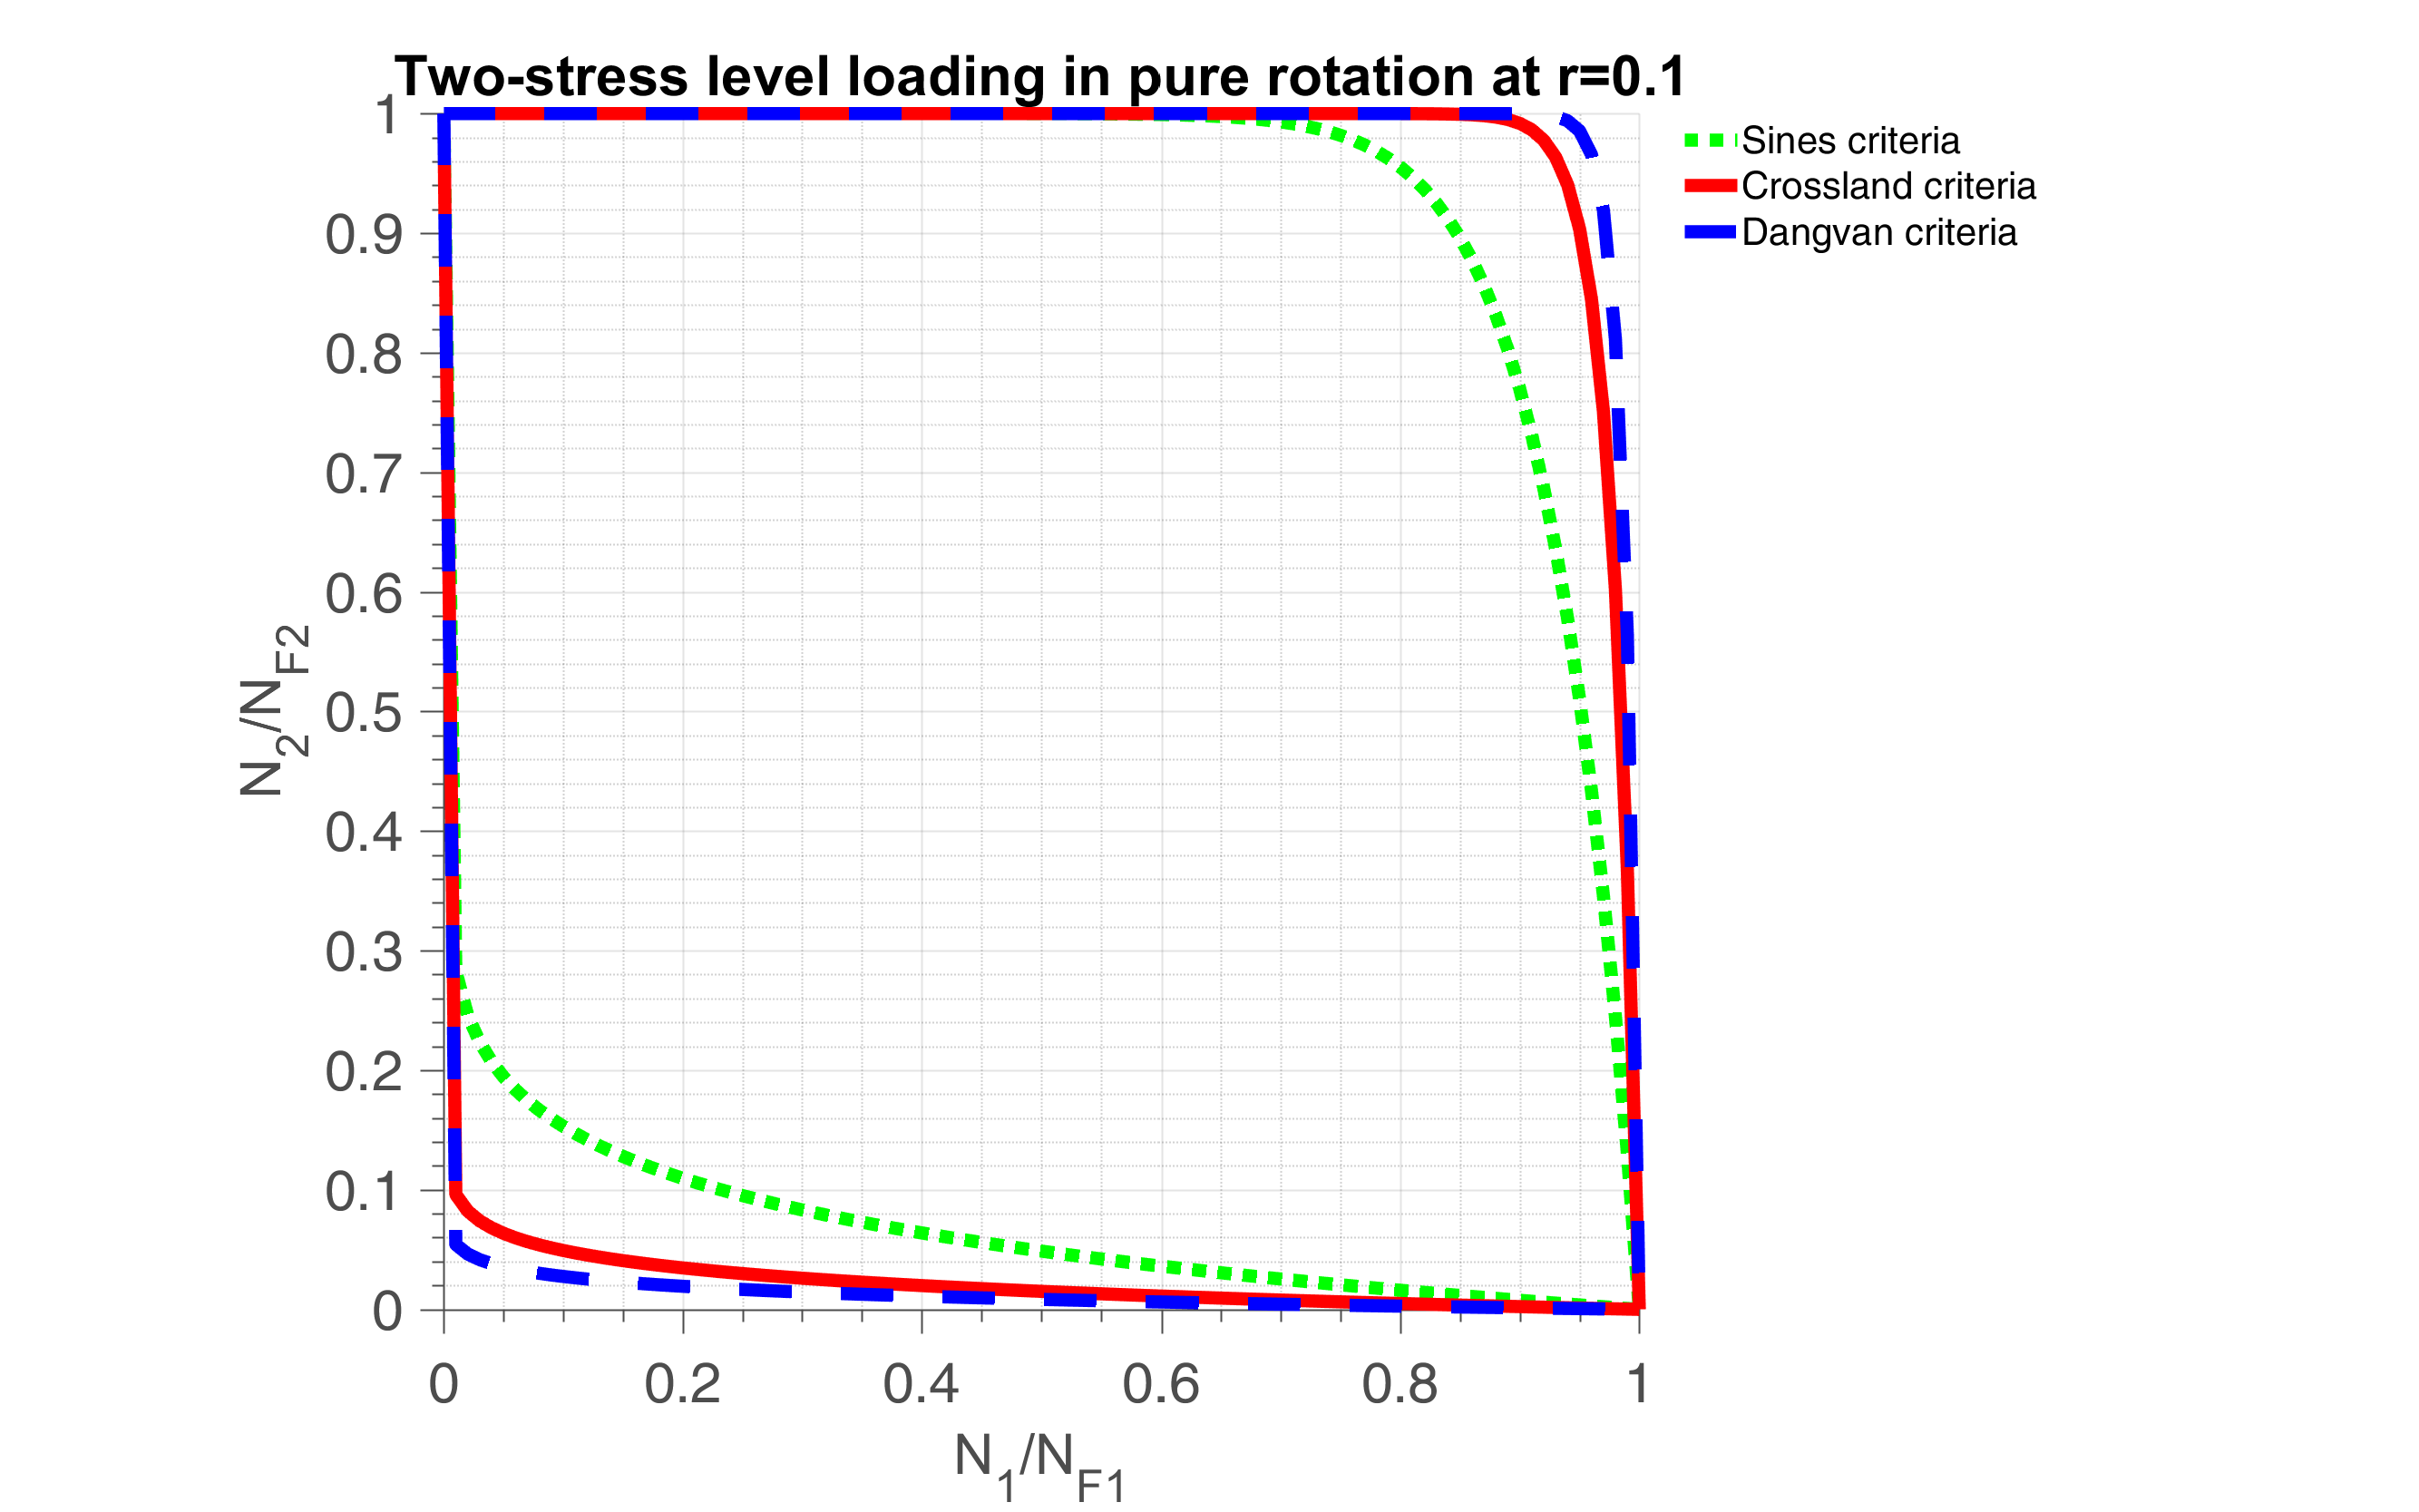
\includegraphics[width=\textwidth]{figures//2stressR.png} 
	\caption{Two-stress level loading in pure rotation at r=0.1. The lower curve displays the relative proportion of cycles in high-low sequence, the upper curve displays the same information in a low-high sequence}
	\label{2stressR}
\end{figure}

\newpage
\subsection{Test on 4-point bending}
From the fatigue zone we select $y=3$ to study. We select here:

$s_{-1}=f_{-1}=0.8MPa$,

$\sigma_{u}=1.67MPa$ 

$\gamma=6$

The $A_{\uppercase\expandafter{\romannumeral2}}-N_F$ figure is shown in \figref{JNbending}.
\begin{figure}[!h]
	\centering
	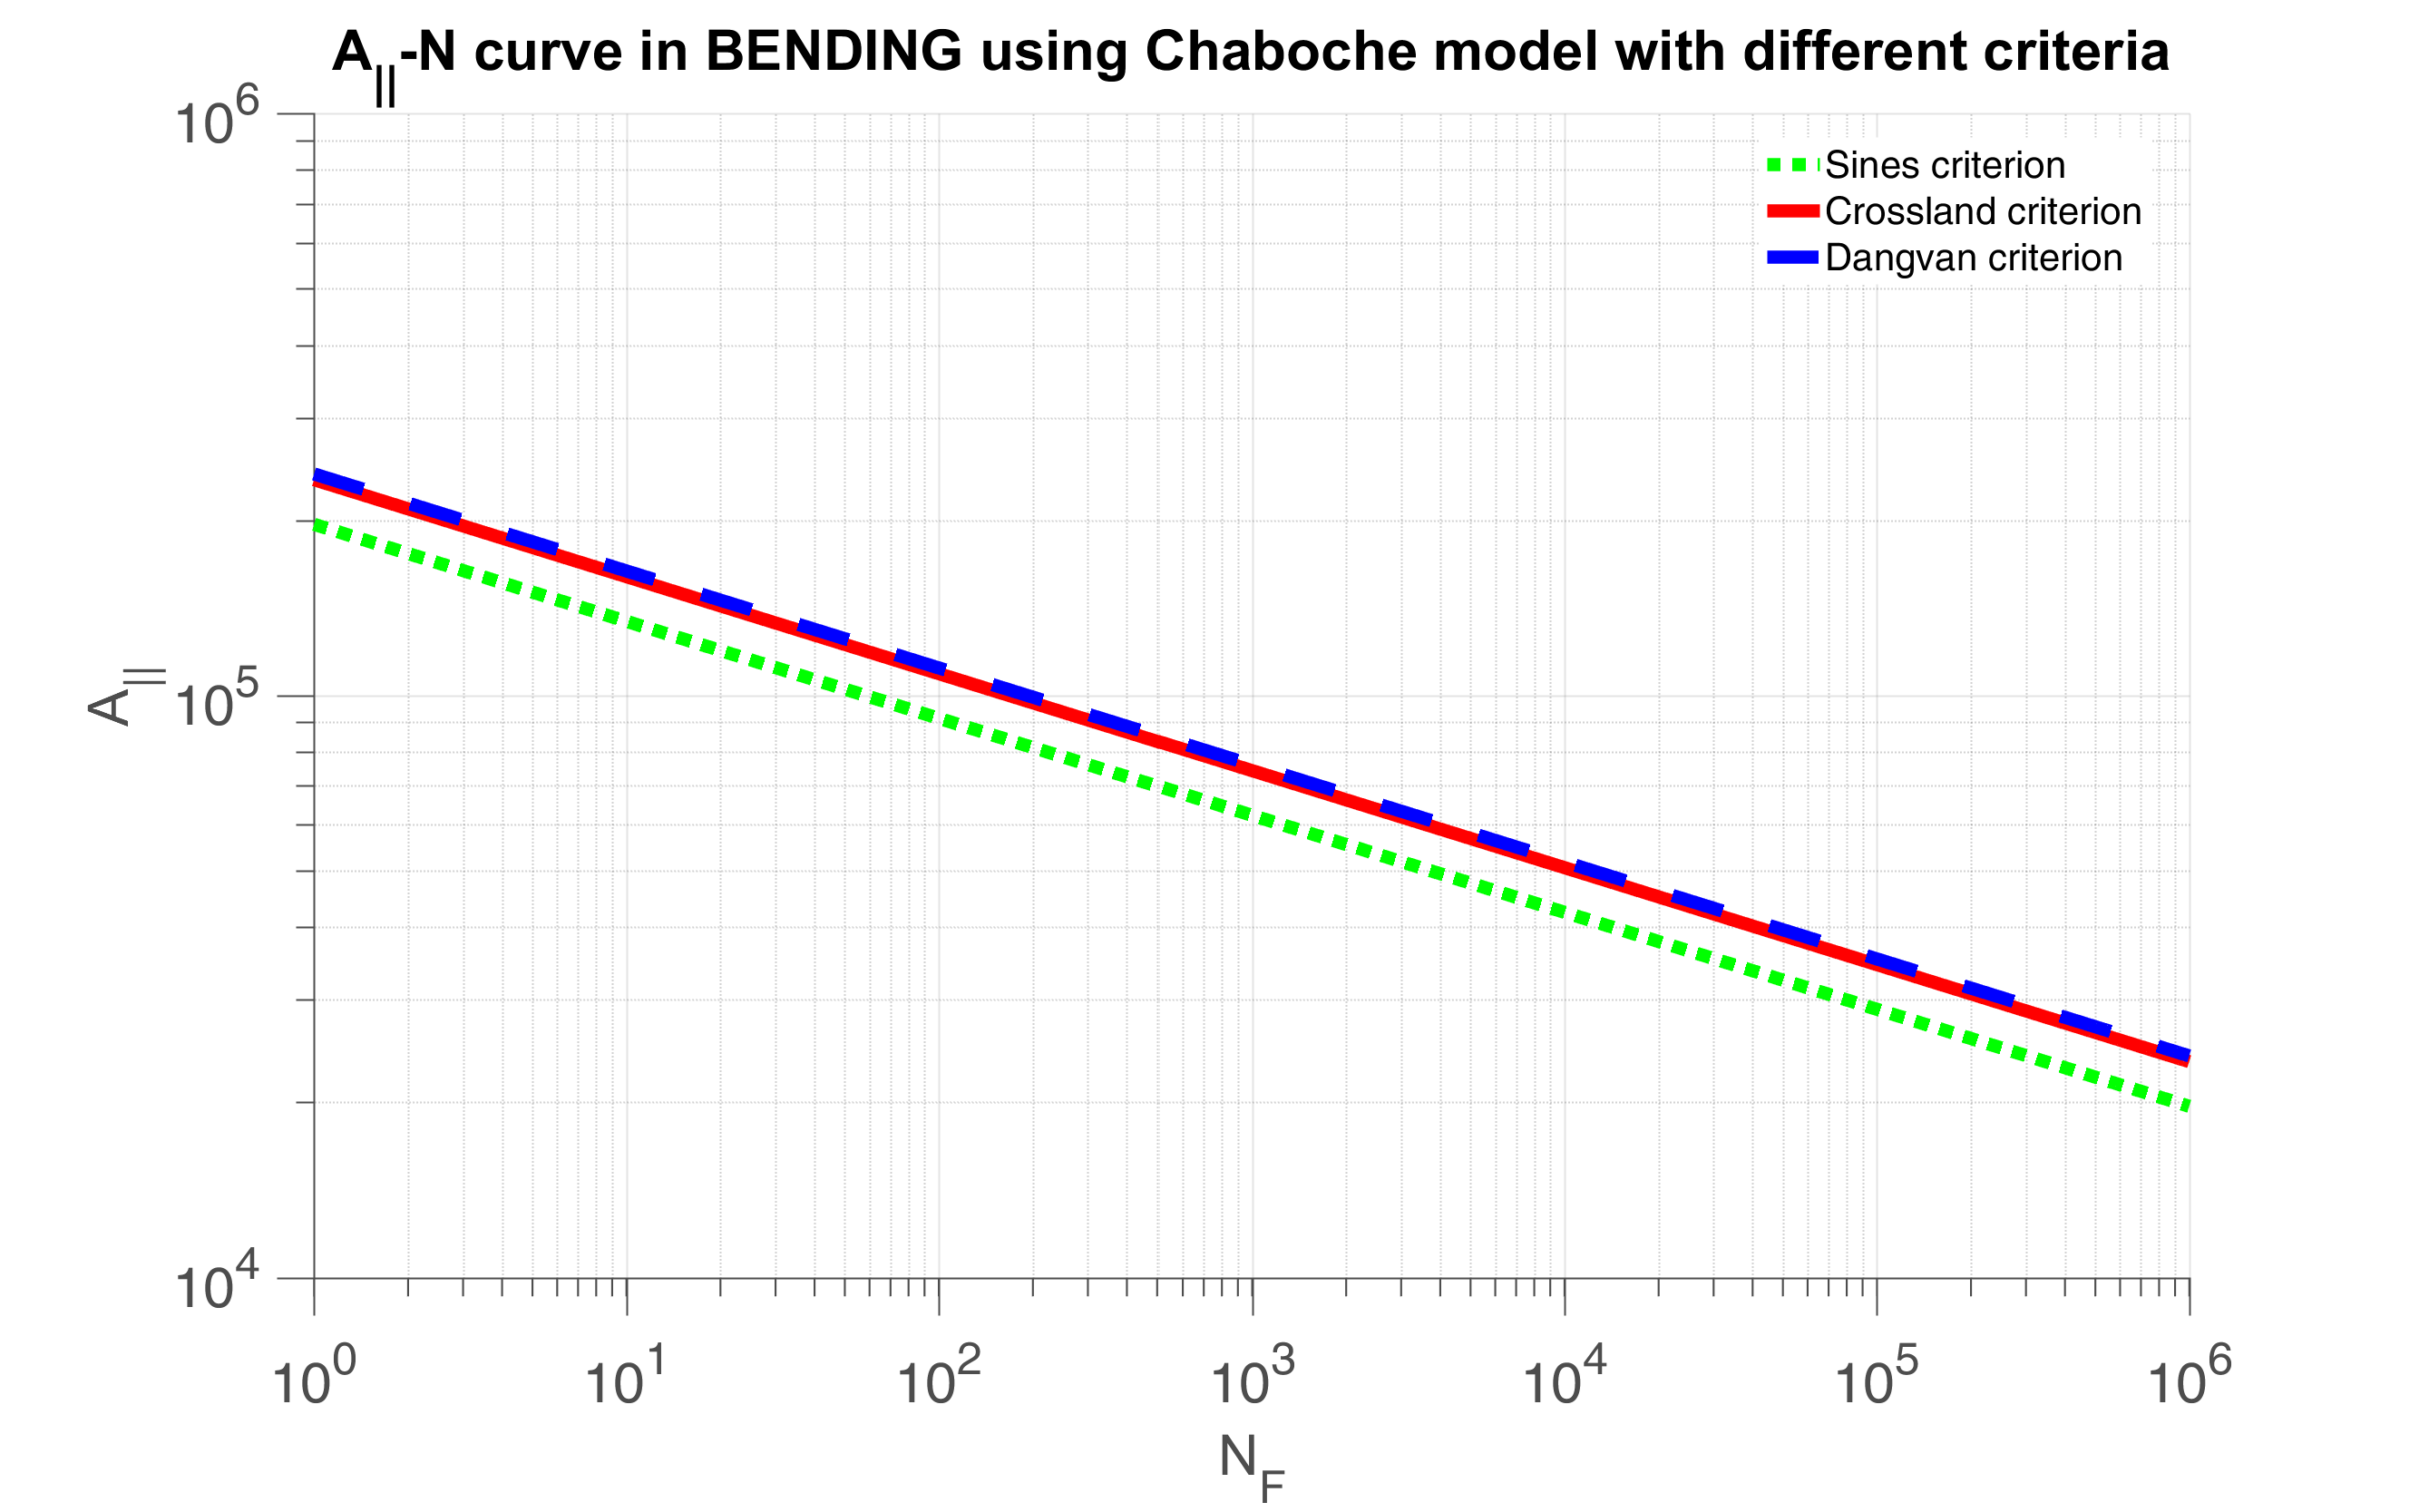
\includegraphics[width=\textwidth]{figures//JNbending.png} 
	\caption{$A_{\uppercase\expandafter{\romannumeral2}}-N_F$ curve in 4-point bending at y=3}
	\label{JNbending}
\end{figure}

In 4-point bending,we assume the first and second loading are respectively $F_1=1E6 N$ and $F_2=0.8E6 N$. 

\vspace{6pt}
$\sqrt{J_{2a_1}}=7.2194E5 Pa$

\vspace{6pt}
$\sqrt{J_{2a_2}}=5.7755E5 Pa$

\vspace{6pt}
$P_{m_1}=3.9298E5 Pa$

\vspace{6pt}
$P_{m_2}=3.1438E5 Pa$

Substituting the above to Eq.\eqref{eq.etachaboche} we can get $\eta$ in High-Low sequence:
and in Low-High sequence as shown in Table.\ref{tab.etabending}:
\begin{table}[!h]
	\centering
	\begin{tabular}{llll}
		\hline
		$\eta$ value   & Sines  & Crossland & Dang Van \\ \hline
		High-low & 0.3174 & 0.1894    &  0.1659   \\
		Low-high & 3.1510 & 5.2794   & 6.0280  \\ \hline
	\end{tabular}
	\caption{$\alpha$ induced sequence effect parameter $\eta$ value with different criteria in bending}
	\label{tab.etabending}
\end{table}

The predicted results are shown in \figref{2stressB}.

\begin{figure}[!h]
	\centering
	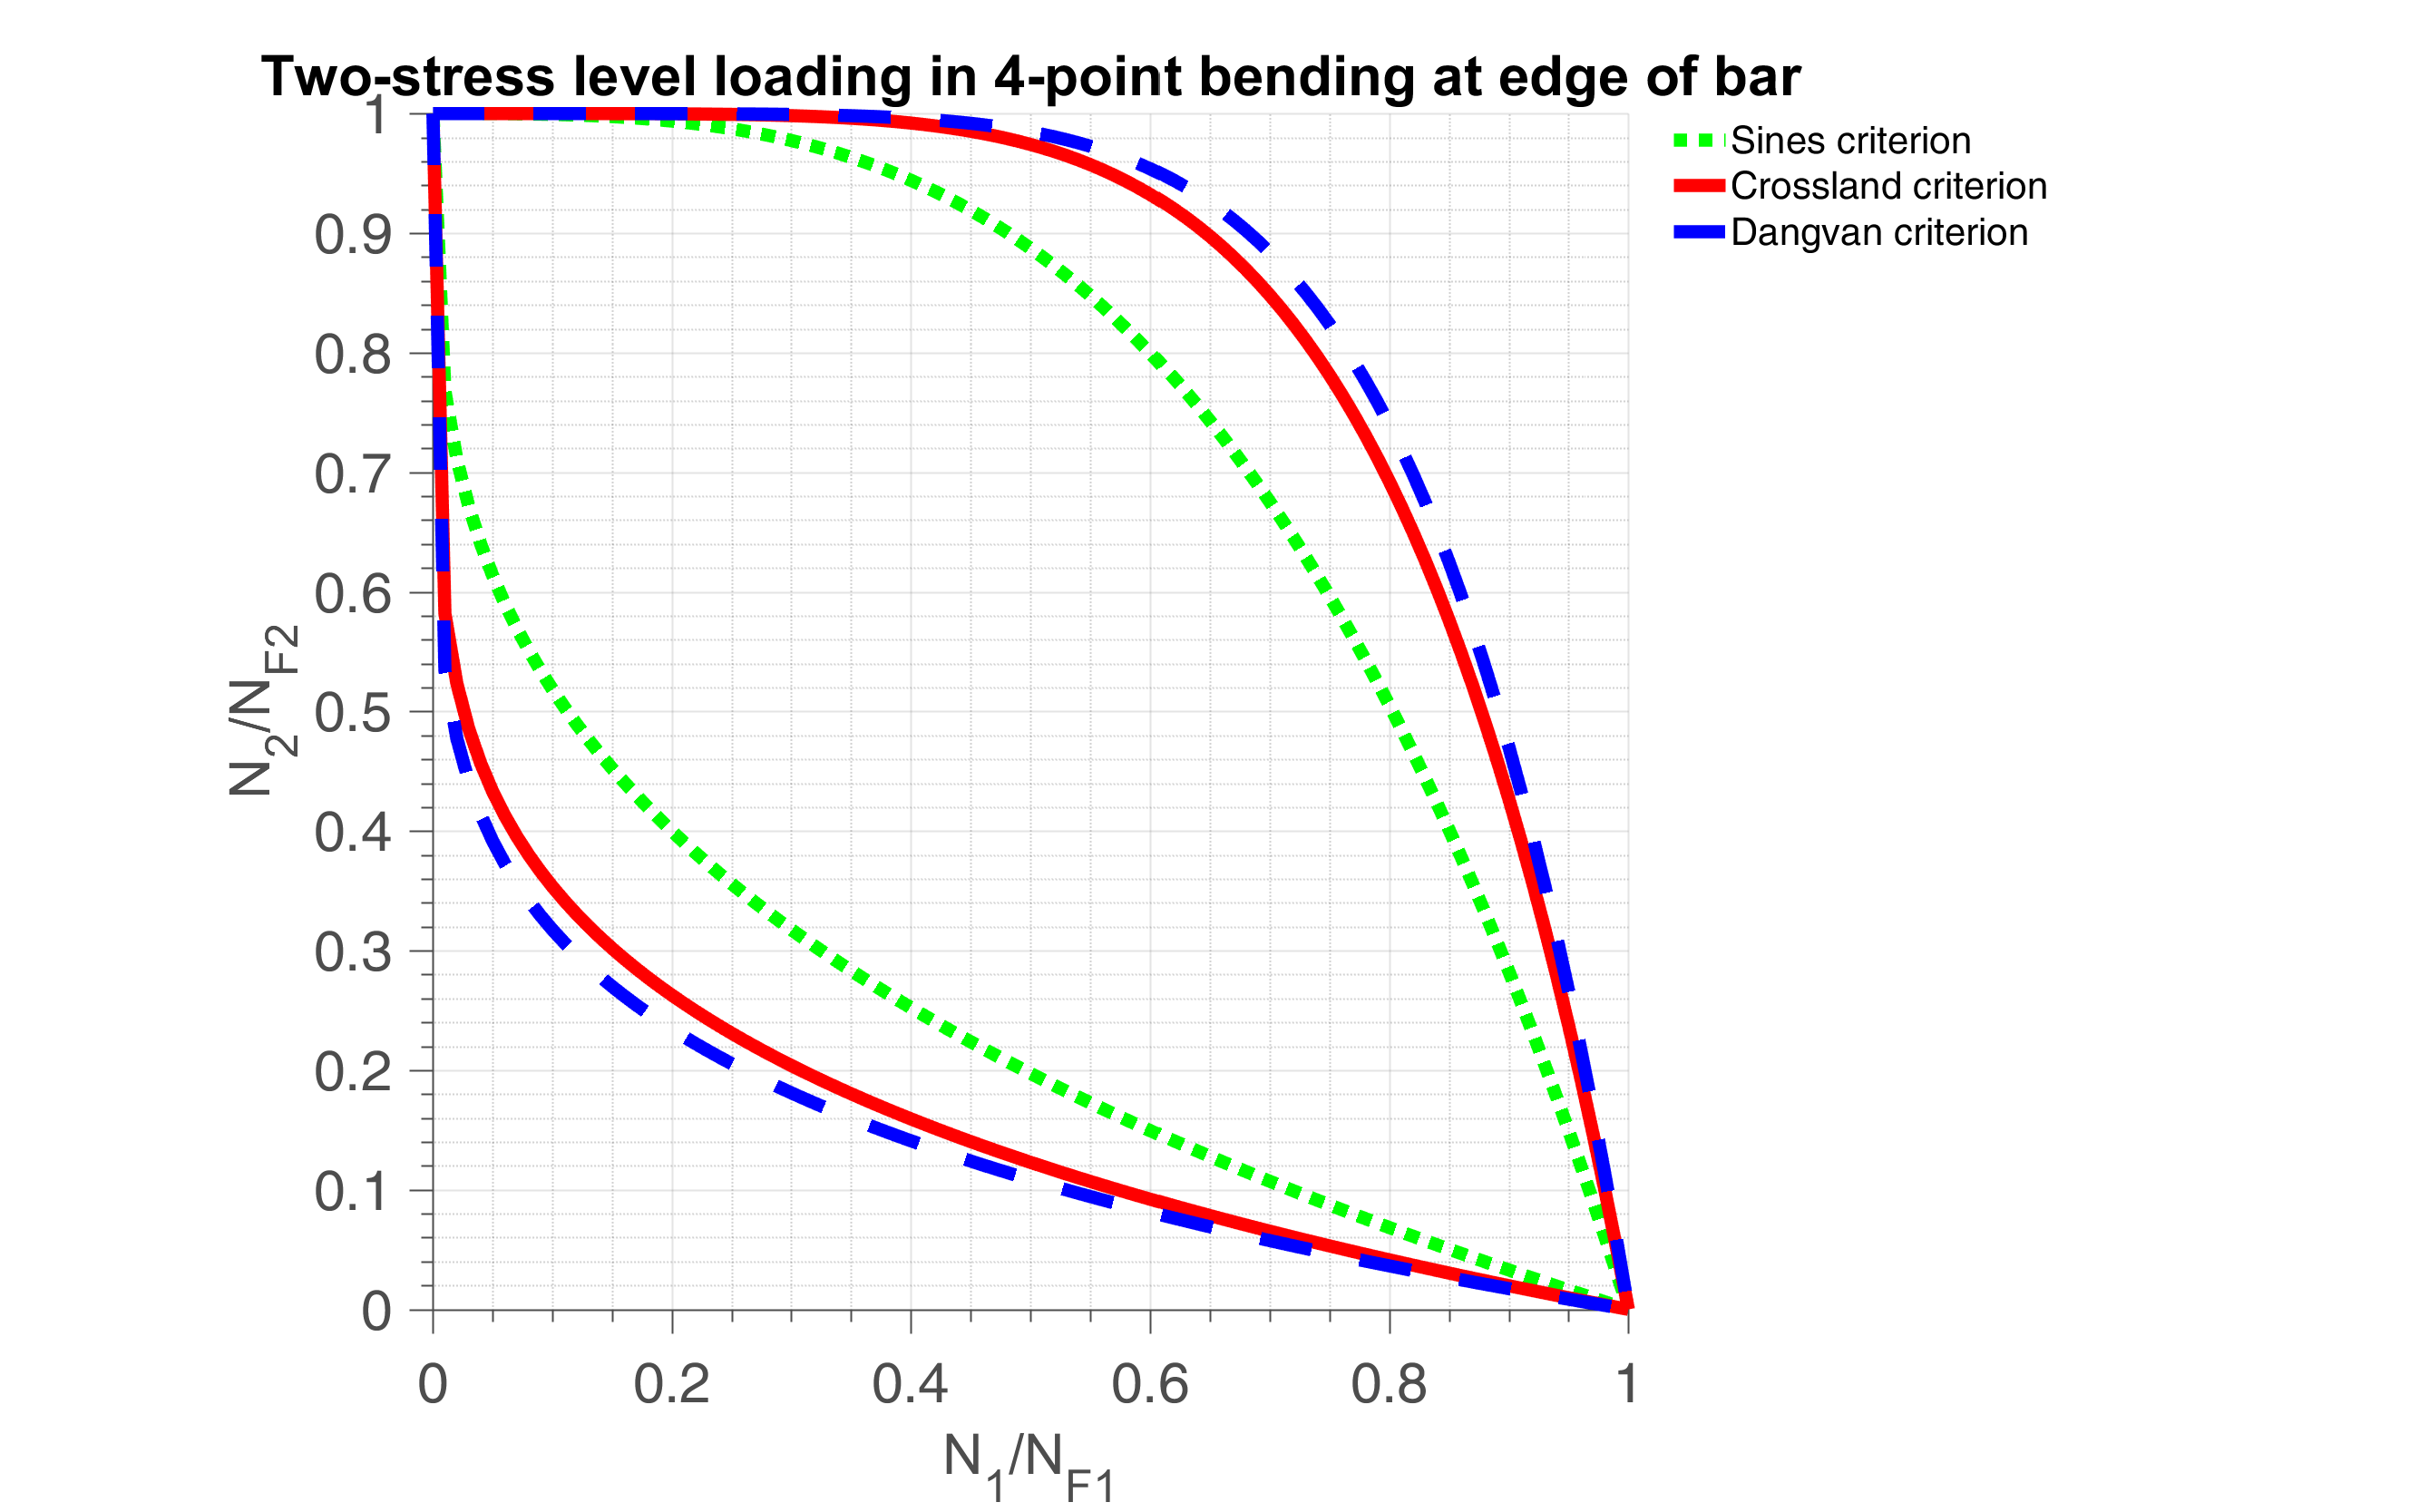
\includegraphics[width=\textwidth]{figures//2stressB.png} 
	\caption{Two-stress level loading in 4-point bending at y=3. The lower curve displays the relative proportion of cycles in high-low sequence, the upper curve displays the same information in a low-high sequence}
	\label{2stressB}
\end{figure}

\newpage
\subsection{Test on rotative bending}
From the fatigue zone we select $r=0.5$ as the radius to study. 
The $A_{\uppercase\expandafter{\romannumeral2}}-N_F$ figure is shown in \figref{JNRB}.

\begin{figure}[!h]
	\centering
	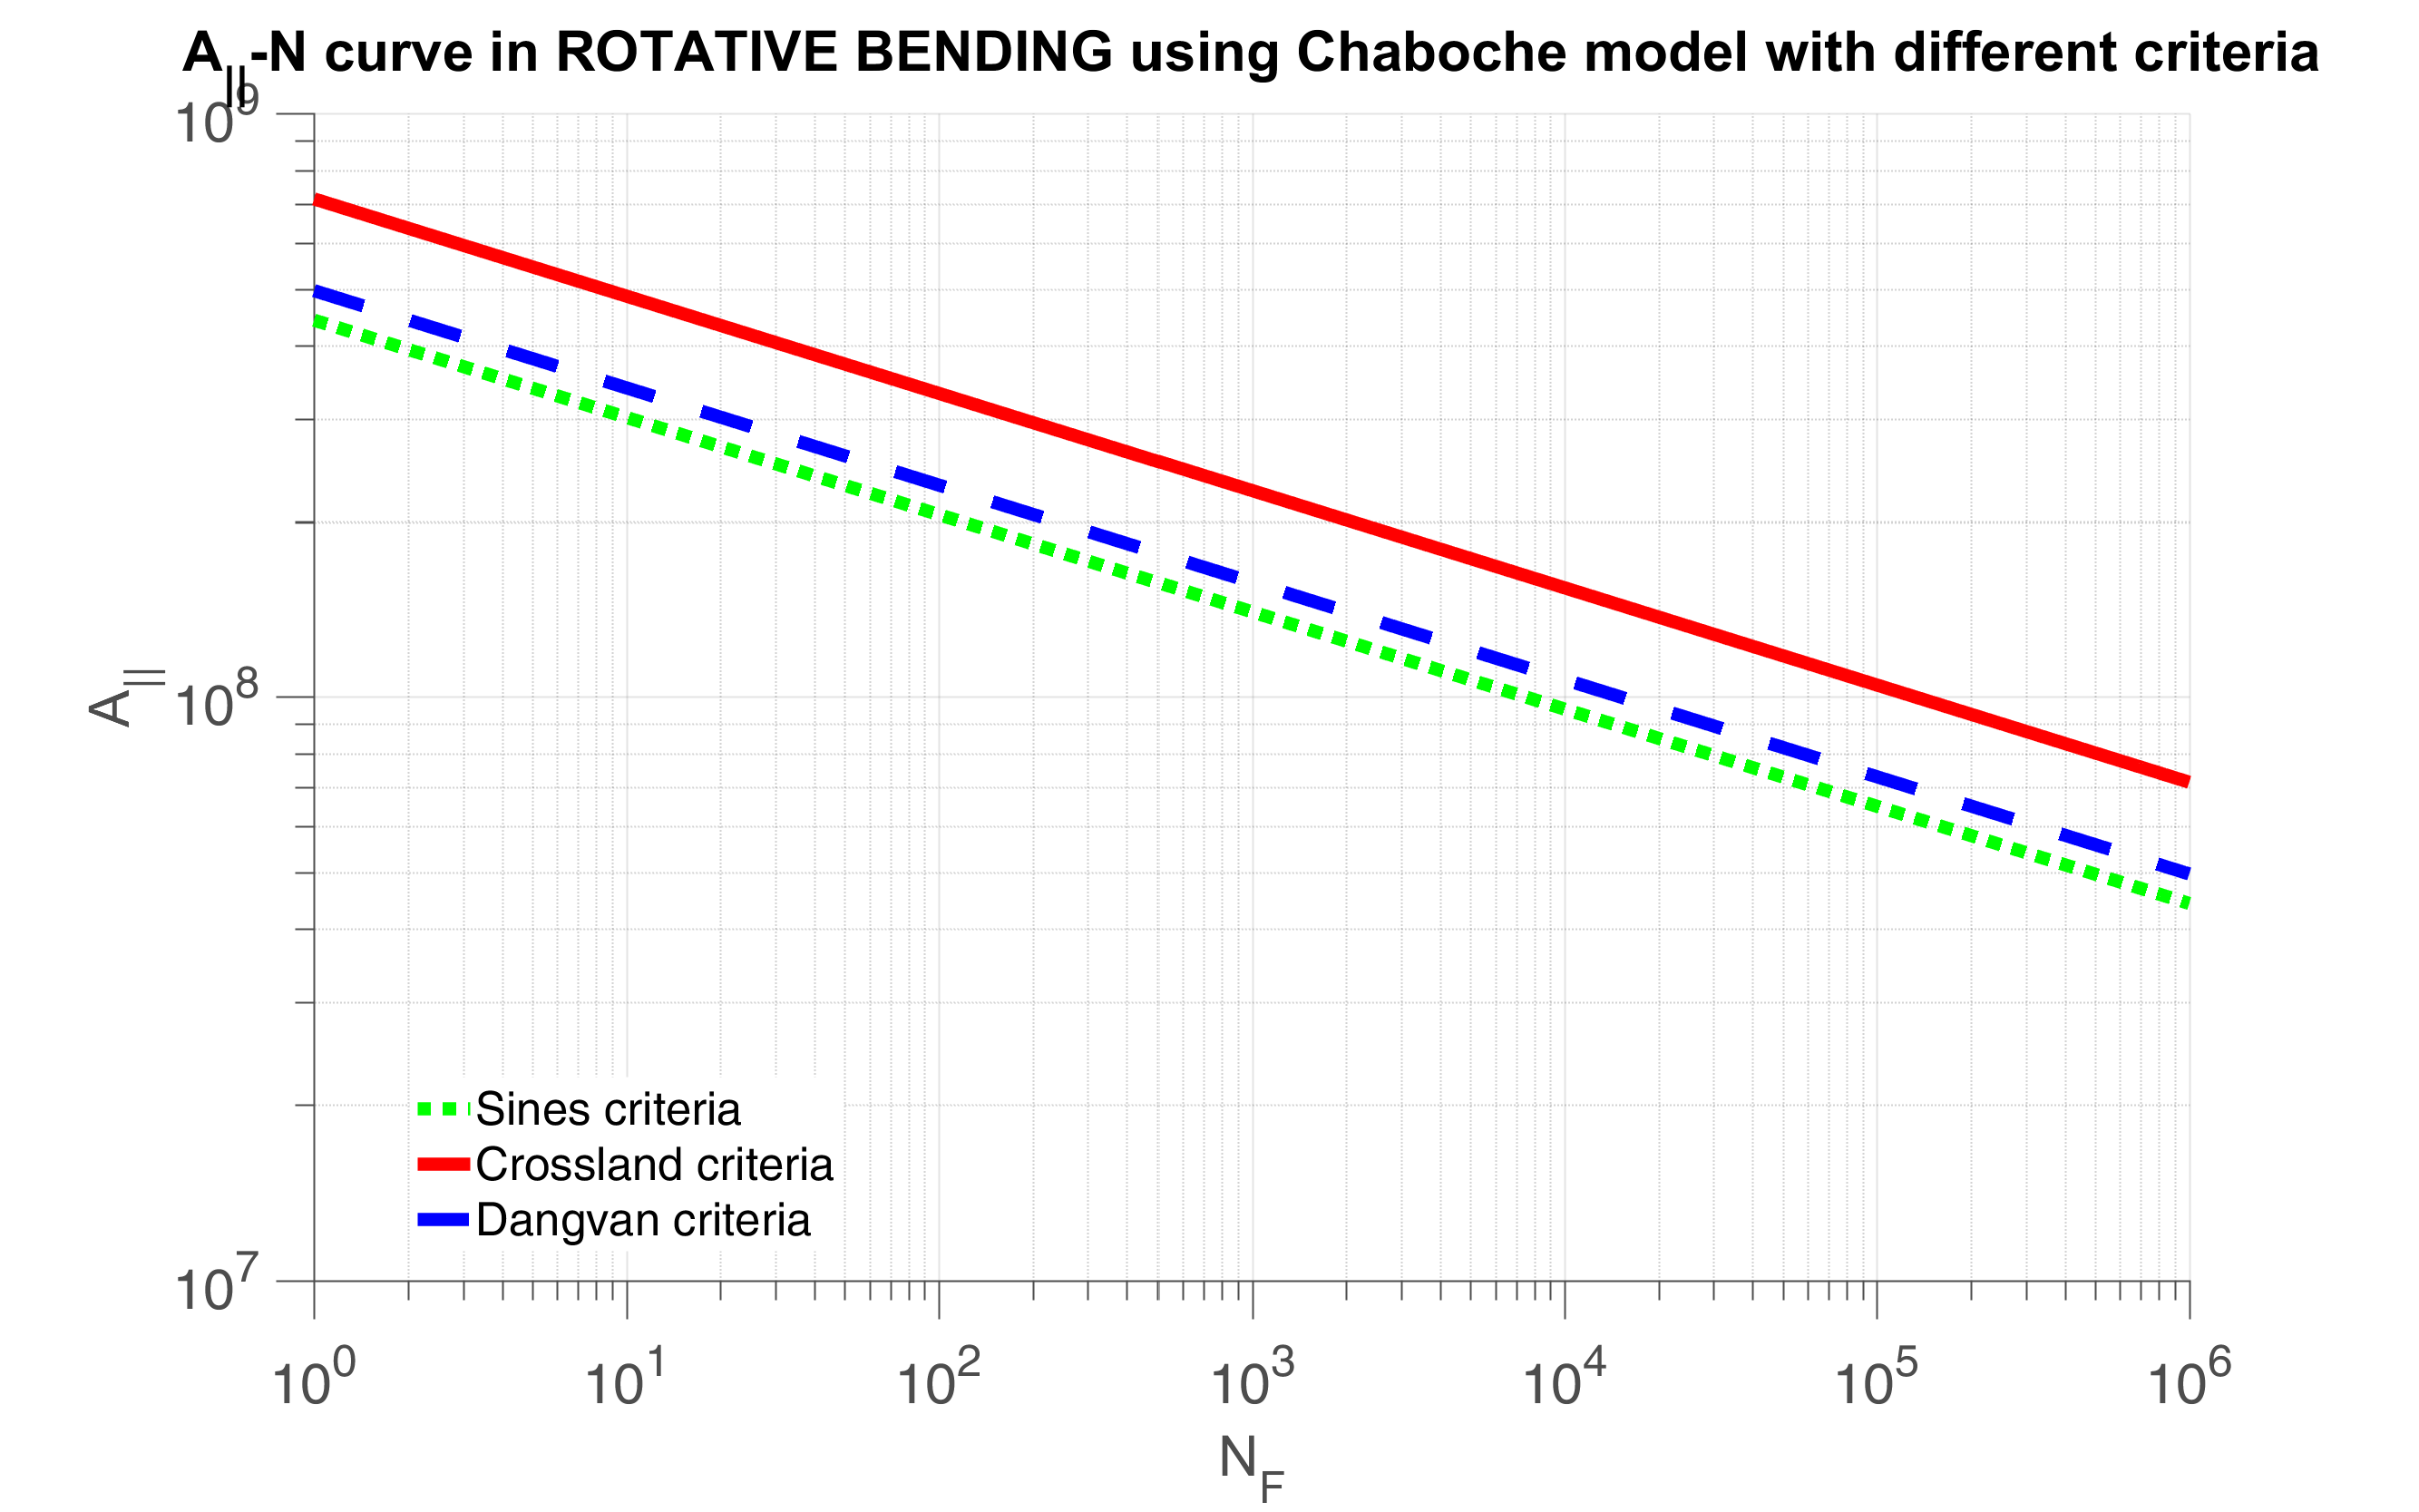
\includegraphics[width=\textwidth]{figures//JNRB.png} 
	\caption{$A_{\uppercase\expandafter{\romannumeral2}}-N_F$ curve in rotative bending at r=3}
	\label{JNRB}
\end{figure}

In rotative bending,we assume the rotating speed are $w=5rpm$. The applied force are respectively $F=9E5 N$ and $F=3E5 N$. We select:

$s_{-1}=f_{-1}=400MPa$, $\sigma_{u}=1000MPa$

\vspace{6pt}
$\sqrt{J_{2a_1}}=7.0226E8 Pa$

\vspace{6pt}
$\sqrt{J_{2a_2}}=6.6454E8 Pa$

\vspace{6pt}
$P_{m_1}=6.8921E8 Pa$

\vspace{6pt}
$P_{m_2}=7.1700E8 Pa$

Substituting the above to Eq.\eqref{eq.eta} we can get $\eta$ in High-Low sequence:
and in Low-High sequence as shown in Table.\ref{tab.etarb}:
\begin{table}[!h]
	\centering
	\begin{tabular}{llll}
		\hline
		$\eta$ value   & Sines  & Crossland & Dang Van \\ \hline
		High-low & 0.7170 &  0.7392 &   0.6608   \\
		Low-high & 1.3947 & 1.3528   &  1.5133  \\ \hline
	\end{tabular}
	\caption{$\alpha$ induced sequence effect parameter $\eta$ value with different criteria in rotative bending}
	\label{tab.etarb}
\end{table}

The predicted results are shown in \figref{2stressRB} which are very close to a situation of linear damage accumulation.

\begin{figure}[!h]
	\centering
	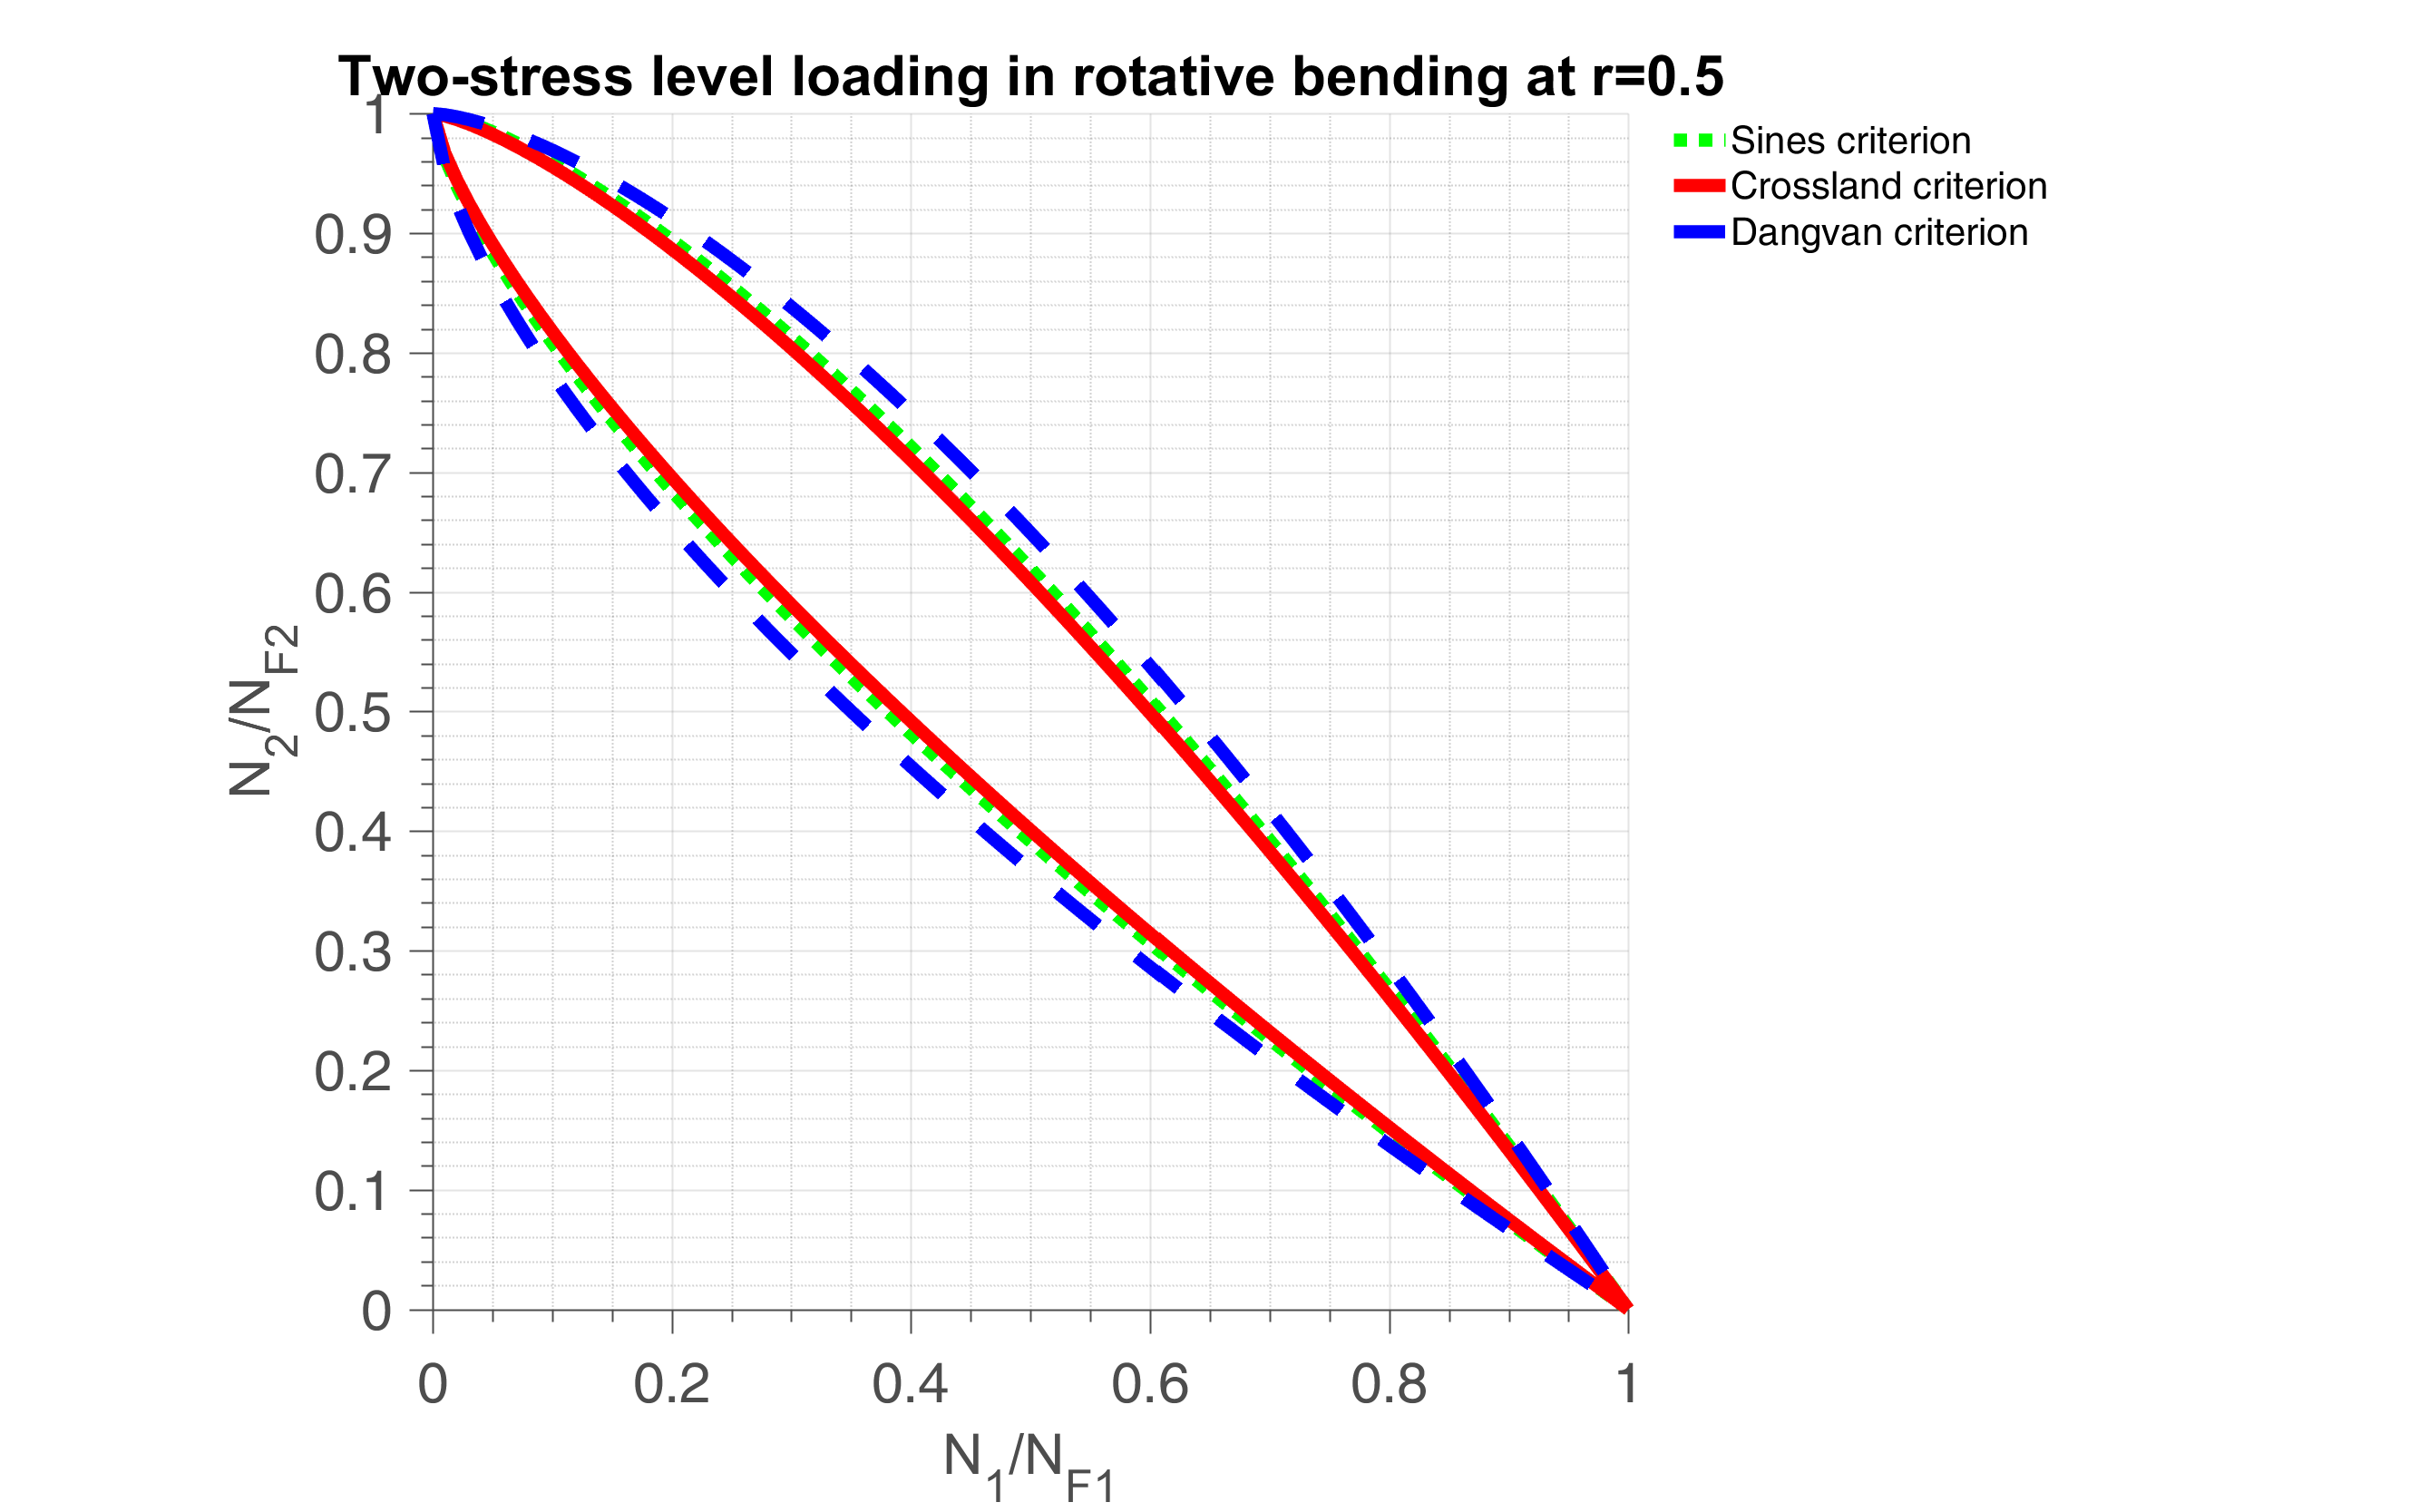
\includegraphics[width=\textwidth]{figures//2stressRB.png} 
	\caption{Two-stress level loading in rotative bending at r=0.5. The lower curve displays the relative proportion of cycles in high-low sequence, the upper curve displays the same information in a low-high sequence}
	\label{2stressRB}
\end{figure}
\clearpage

\textbf{Discussion}

The Chaboche law is based on this assumption: fatigue damage occurs and accumulates only when the loading stress is higher than its fatigue limit. Therefor, Eq.\eqref{chabochemulti} neglects the damage contribution of the loading stress which is lower than the fatigue limit. According to some experimental results such as: Lu and Zheng \cite{xi2008strengthening} \cite{xi2009strengthening} \cite{xi2009changes}, Sinclair \cite{sinclair1952investigation}, and Makajima et al. \cite{nakajima2007coaxing}, however, it appears that the damage of low amplitude loads is one
of the main reasons for prediction errors. 

Impurities in the material affect the fatigue life. So does the material's hardness, and especially its surface condition. How the components were heat-treated in the factory is another factor. The operating temperature makes a difference, too. Worse still is the structural component's shape: notches and sharp corners create concentrations of stress that can initiate cracks. Thus further studies should be carried out concerning these factors whilst studying damage accumulation.

\section{Cycle Counting Method}
\label{sec:5.1}
Whatever damage accumulation law is used, whatever fatigue criterion is used(Sines, Crossland, Dang Van,...), up to now all fatigue prediction which have been presented are based on the notion of cyclic loads of different amplitudes applied successively. How do we identify those cycles in a random loading history?

In this framework, a counting method is a method for identifying a statistical event
in a random loading sequence. This event can be, for example, extrema,
ranges or cycles of the signal. A method of counting stress cycles determines
therefore the number or the density of presence of the stress cycles in the loading signal.
In other words, the counting method consists in discretizing the loading sequence
variable in simple elementary cycles easy to implement in any forecasting process
of fatigue life. Indeed, each elementary cycle, extracted from the sequence of
load, is denoted by its amplitude and its mean value to which corresponds one
well-defined lifetime. Then, the elementary damage of the extracted cycle is calculated using
a rule of damage. The process repeats along the sequence studied to evaluate
the total damage by means of an accumulation law, and consequently to determine the number of
sequences at break.

Some methods of counting have been developed by the experts. They all lead to different results and therefore, for some, to errors in the calculation of the duration of life. We can cite by way of example six major families of counting techniques,
described in various works \cite{ASTM1985}:

\vspace{6pt}
\noindent
- the counting of the loading time,\\
- the counting of extrema between two passages by the mean value,\\
- the counting of areas,\\
- the counting of paired ranges,\\
- the counting of overflows,\\
- rainflow cycle counting, say ``the drop of water."
\vspace{6pt}

The object of all cycle counting methods is to compare the effect of variable amplitude load histories to fatigue data and curves obtained with simple constant amplitude load cycles. Rainflow counting is a process to obtain cyclic data of complex loading. Its name comes from the original description from the Japanese researchers Matsuiski and Endo where they describe the process in terms of rain falling off a pagoda style roof. A more insightful description based on cyclic plasticity is usually used to explain the method.

\begin{figure}[!h]
	\centering
	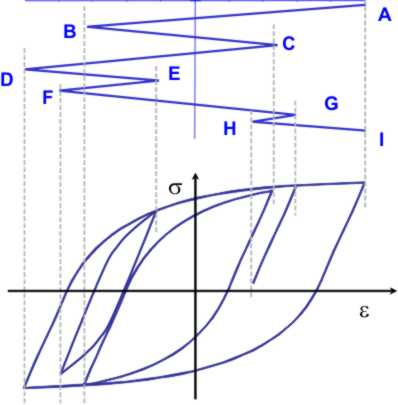
\includegraphics[width=0.4\textwidth]{figures//rainflow.jpg} 
	\caption{Complex Cyclic Loading}
	\label{rainflow}
\end{figure}

In \figref{rainflow}(retrieved from https://www.efatigue.com/variable/background/rainflow.html) a simple loading history ( points A - I ) is plotted vertically so that it resembles a Japanese pagoda. The resulting deformation, stresses and strains, is plotted directly below the loading history. In the lower part of the figure, four cycles are easily identified. One large overall cycle, one intermediate cycle in the center of the plot, and two smaller cycles. Each cycle has its own strain range and mean stress. From a deformation viewpoint the process proceeds as follows. Start at A, the maximum strain, and unload the material to B. Then reload to point C and unload to D. When the material reaches the strain at point B during the unloading from C to D the material remembers its prior deformation and deforms along a path from A to D as if the event C-D never happened. This is better illustrated in the next part of the loading. Load from D to E and unload to F. Now load from F to G. When the material reaches the strain at point E during the loading from F to G the material remembers its prior deformation and deforms along a path from D to G as if the event E-F never happened. The same process occurs for G-H.

Rainflow counting will identify four cycles, A-D-I, B-C-B, E-F-E and G-H-G. Rainflow counting identifies the major load excursions, for example D to I, and treats subcycles like E-F and G-H as interruptions to the overall loading event D-I.

\vspace{6pt}
The five-step procedure to extract the cyclic data is summarized as follows:

1.  Determine the peaks and valleys of the stress/strain during cycling, and recognize in order to center at the absolute maximum stress (\figref{Reorder}).

2.  Visualize the resulting landscape draining water from the deepest valley (\figref{StressRange}).

3.  Measure total depth drained (stress range) and mean depth (mean stress) of this valley, (\figref{StressRange}), and the number of these cycles in the load history. 

4.  Continue by draining the next lowest (\figref{DrainWater}) and repeat until all valleys are drained. A  Rainflow  cycle is counted if the second segment is vertically shorter than the first and the third segments(i.e. 6-7 is smaller than 5-6 and 7-8).

5.  Use the damage rule to obtain the life from all cycles.

\begin{figure}[!h]
	\centering
	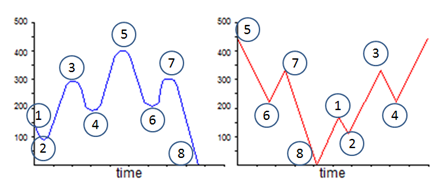
\includegraphics[width=0.6\textwidth]{figures//Reorder.png} 
	\caption{Reorder to Start from Absolute Maximum(retrieved  from ``How to Calculate Fatigue Life When The Load History Is Complex'', February 13, 2015, author: Michael Bak, https://caeai.com/blog/how-calculate-fatigue-life-when-load-history-complex)}
	\label{Reorder}
\end{figure}

\begin{figure}[!h]
	\centering
	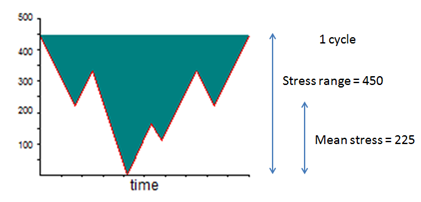
\includegraphics[width=0.6\textwidth]{figures//StressRange.png} 
	\caption{Imagine Filling with Water and Extract Stress Range and Mean Stress(retrieved  from ``How to Calculate Fatigue Life When The Load History Is Complex'', February 13, 2015, author: Michael Bak, https://caeai.com/blog/how-calculate-fatigue-life-when-load-history-complex)}
	\label{StressRange}
\end{figure}

\begin{figure}[!h]
	\centering
	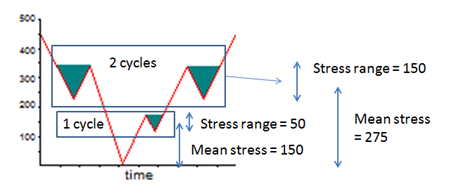
\includegraphics[width=0.6\textwidth]{figures//DrainWater.png} 
	\caption{Drain Water Starting at Lowest Valley and Repeat Cycle Extraction(retrieved  from ``How to Calculate Fatigue Life When The Load History Is Complex'', February 13, 2015, author: Michael Bak, https://caeai.com/blog/how-calculate-fatigue-life-when-load-history-complex)}
	\label{DrainWater}
\end{figure}   

\begin{figure}[!h]
	\centering
	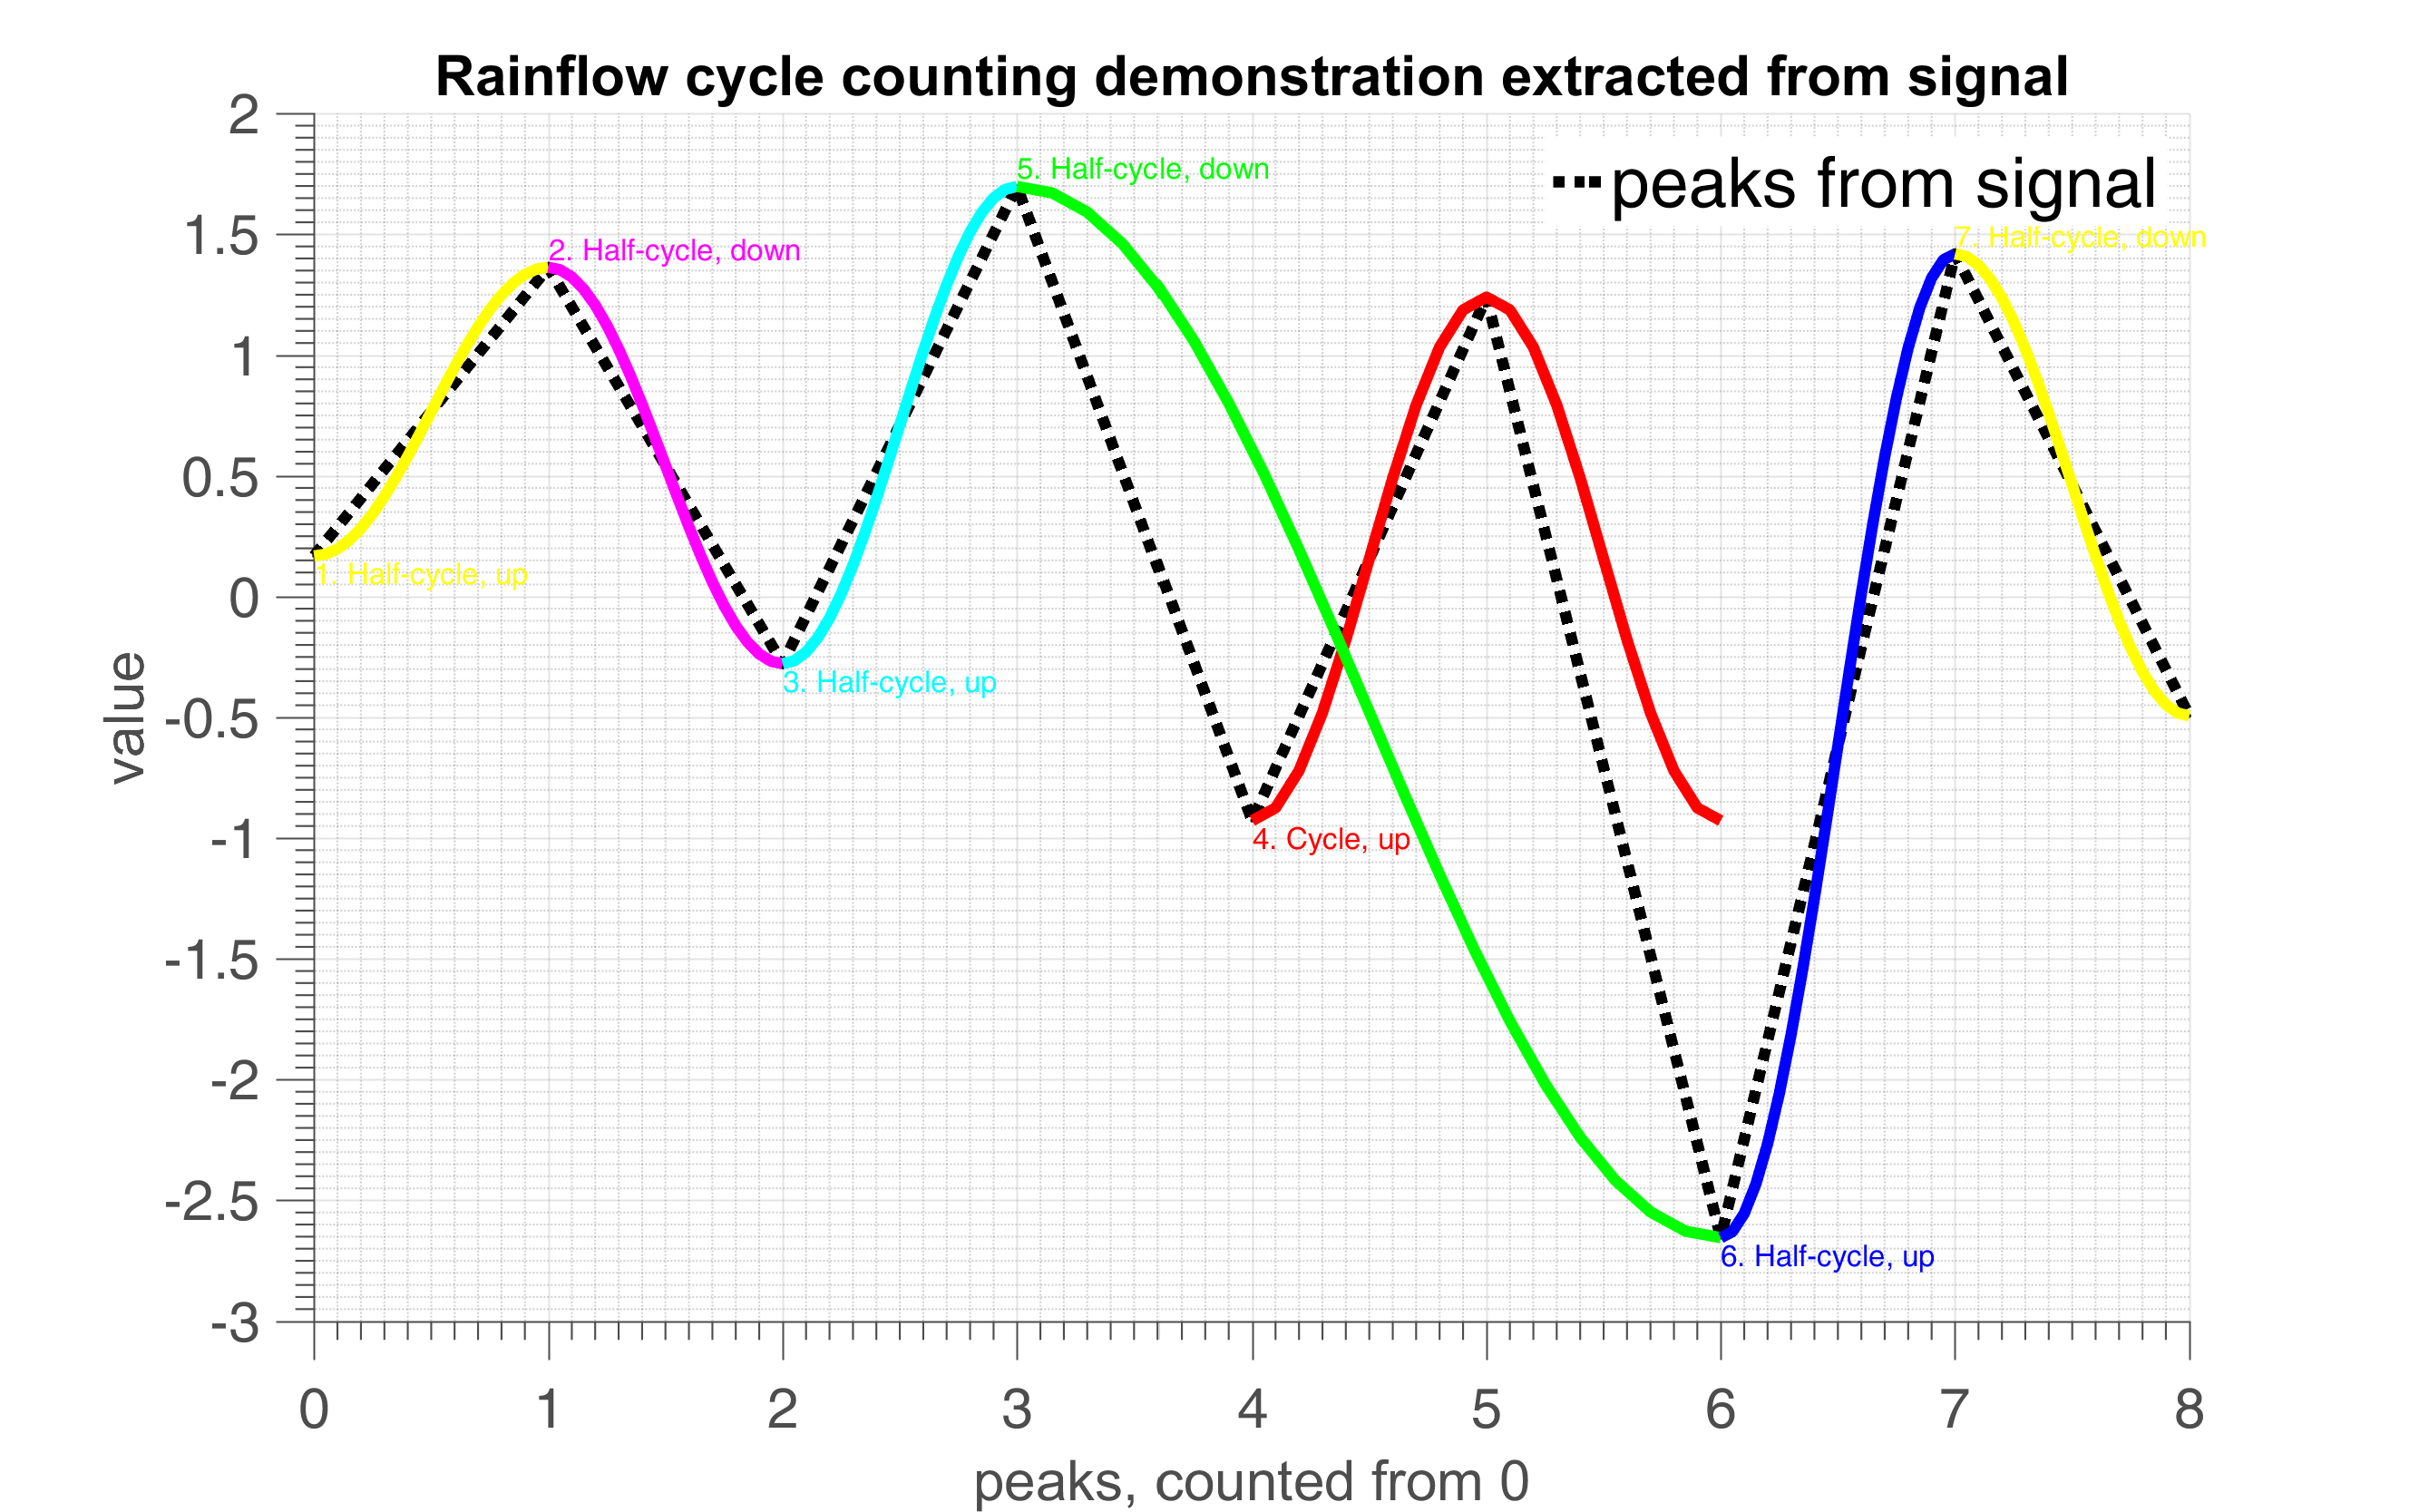
\includegraphics[width=\textwidth]{figures//rfdemo.png} 
	\caption{Rainflow counting method demonstration}
	\label{rfdemo}
\end{figure}  

Once all the cycles have been categorized, the Palmgren-Miner Rule is applied. Even though the linear damage rule ignores sequence effects, it is most widely used because of its simplicity and the fact that though many nonlinear damage models have been developed, unfortunately none can encompass many of the complicating factors encountered during complex variable amplitude loading. As an example, for this case assuming mean stress is ignored, we get in this example:

$$\sum_i \frac{N_i}{N_{F_i}}=\frac{1}{N_{F_{450}}}+\frac{1}{N_{F_{200}}}+\frac{1}{N_{F_{50}}}+...=1.$$

where n is replaced with the number of actual cycles of its corresponding type in the load history, for instance $N_{F_{450}}$ represents the life obtained from the $S-N$ data for a stress range of $450MPa$.  From this equation, the number of total cycles through the entire load history can be found.

The rainflow procedure can be automated so that cyclic content of complex loading can be extracted efficiently.  For example, fatigue computer codes such as $nCode DesignLife$ will accept files of test data, or the input of multiple load steps from a static or transient finite element analysis, and use the rainflow approach to automatically extract the cyclic data.  In addition, $DesignLife$ automates the Palmgrem-Miner Damage Rule calculation to determine number of cycles to failure, with the term cycle here defined as one pass through the entire time history. A computer program in matlab that accomplishes rainflow cycle counting applied to a complex history such as that in \figref{randomdemo} results in a histogram of amplitudes and mean values shown in \figref{randomdemoampl}, \figref{randomdemomean} and \figref{randomdemo3d}.

\begin{figure}[!h]
	\centering
	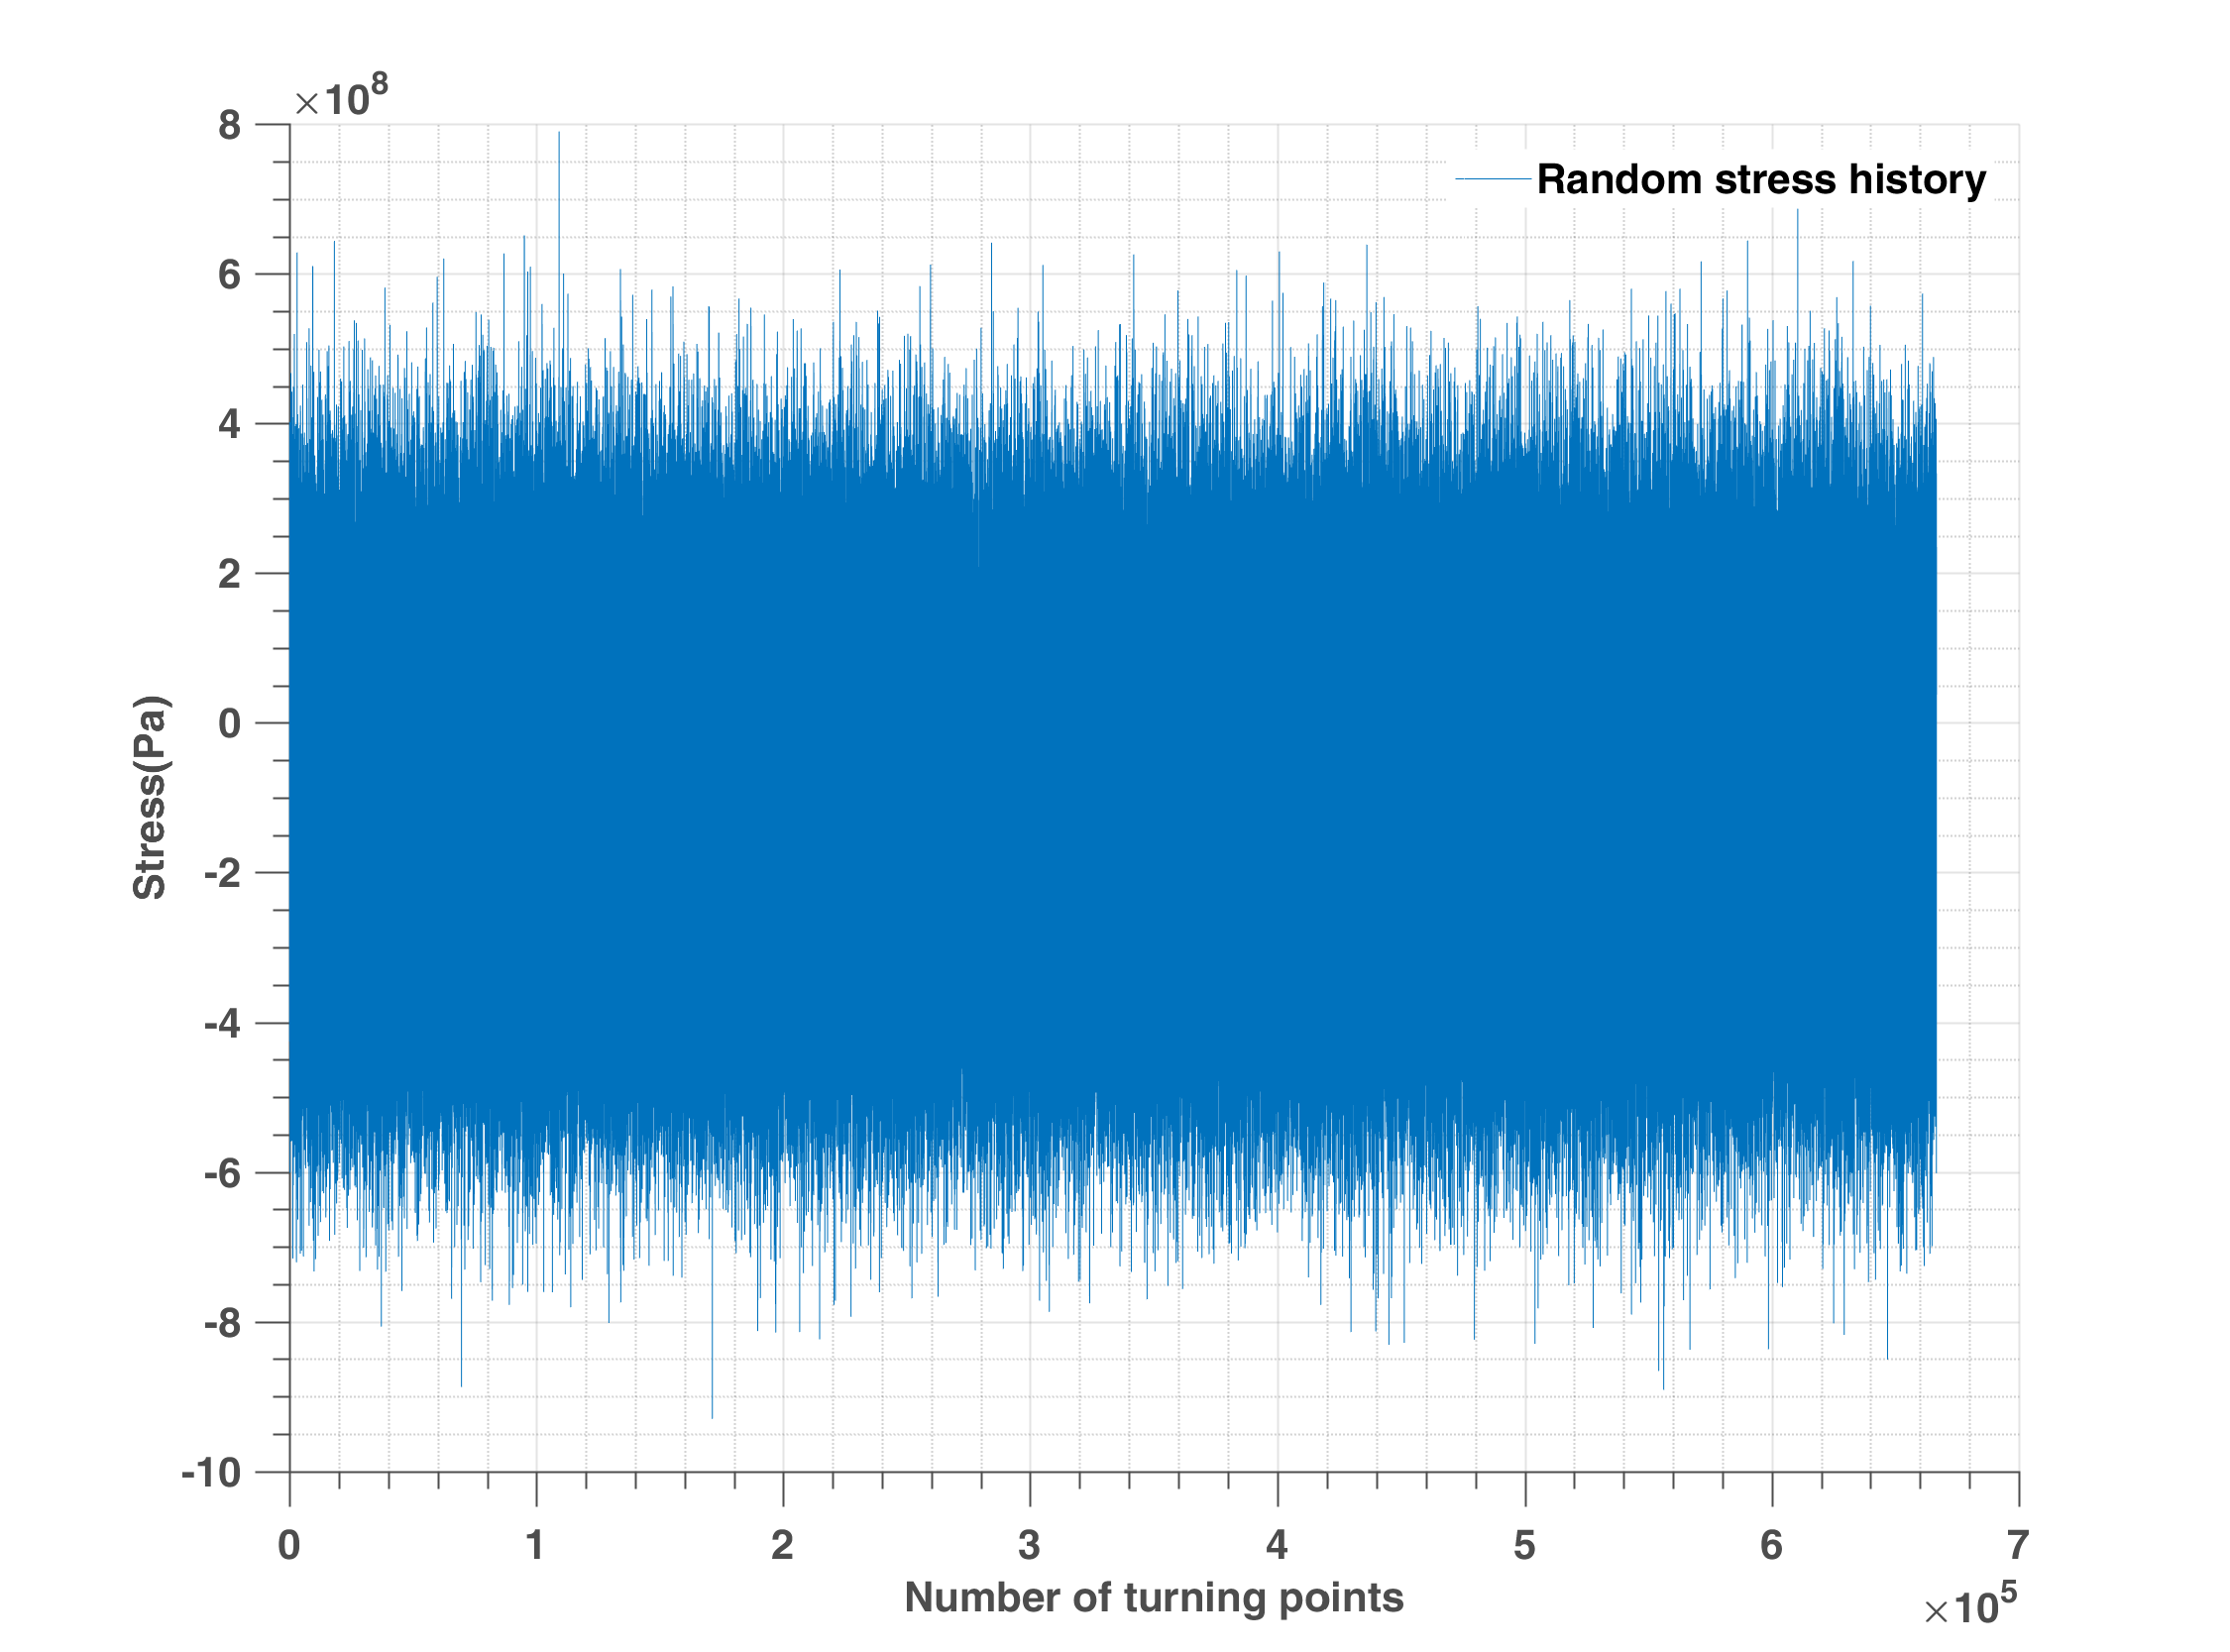
\includegraphics[width=\textwidth]{figures//randomdemo.png} 
	\caption{One million normally distributed random stresses around -100MPa}
	\label{randomdemo}
\end{figure}

\begin{figure}[!h]
	\centering
	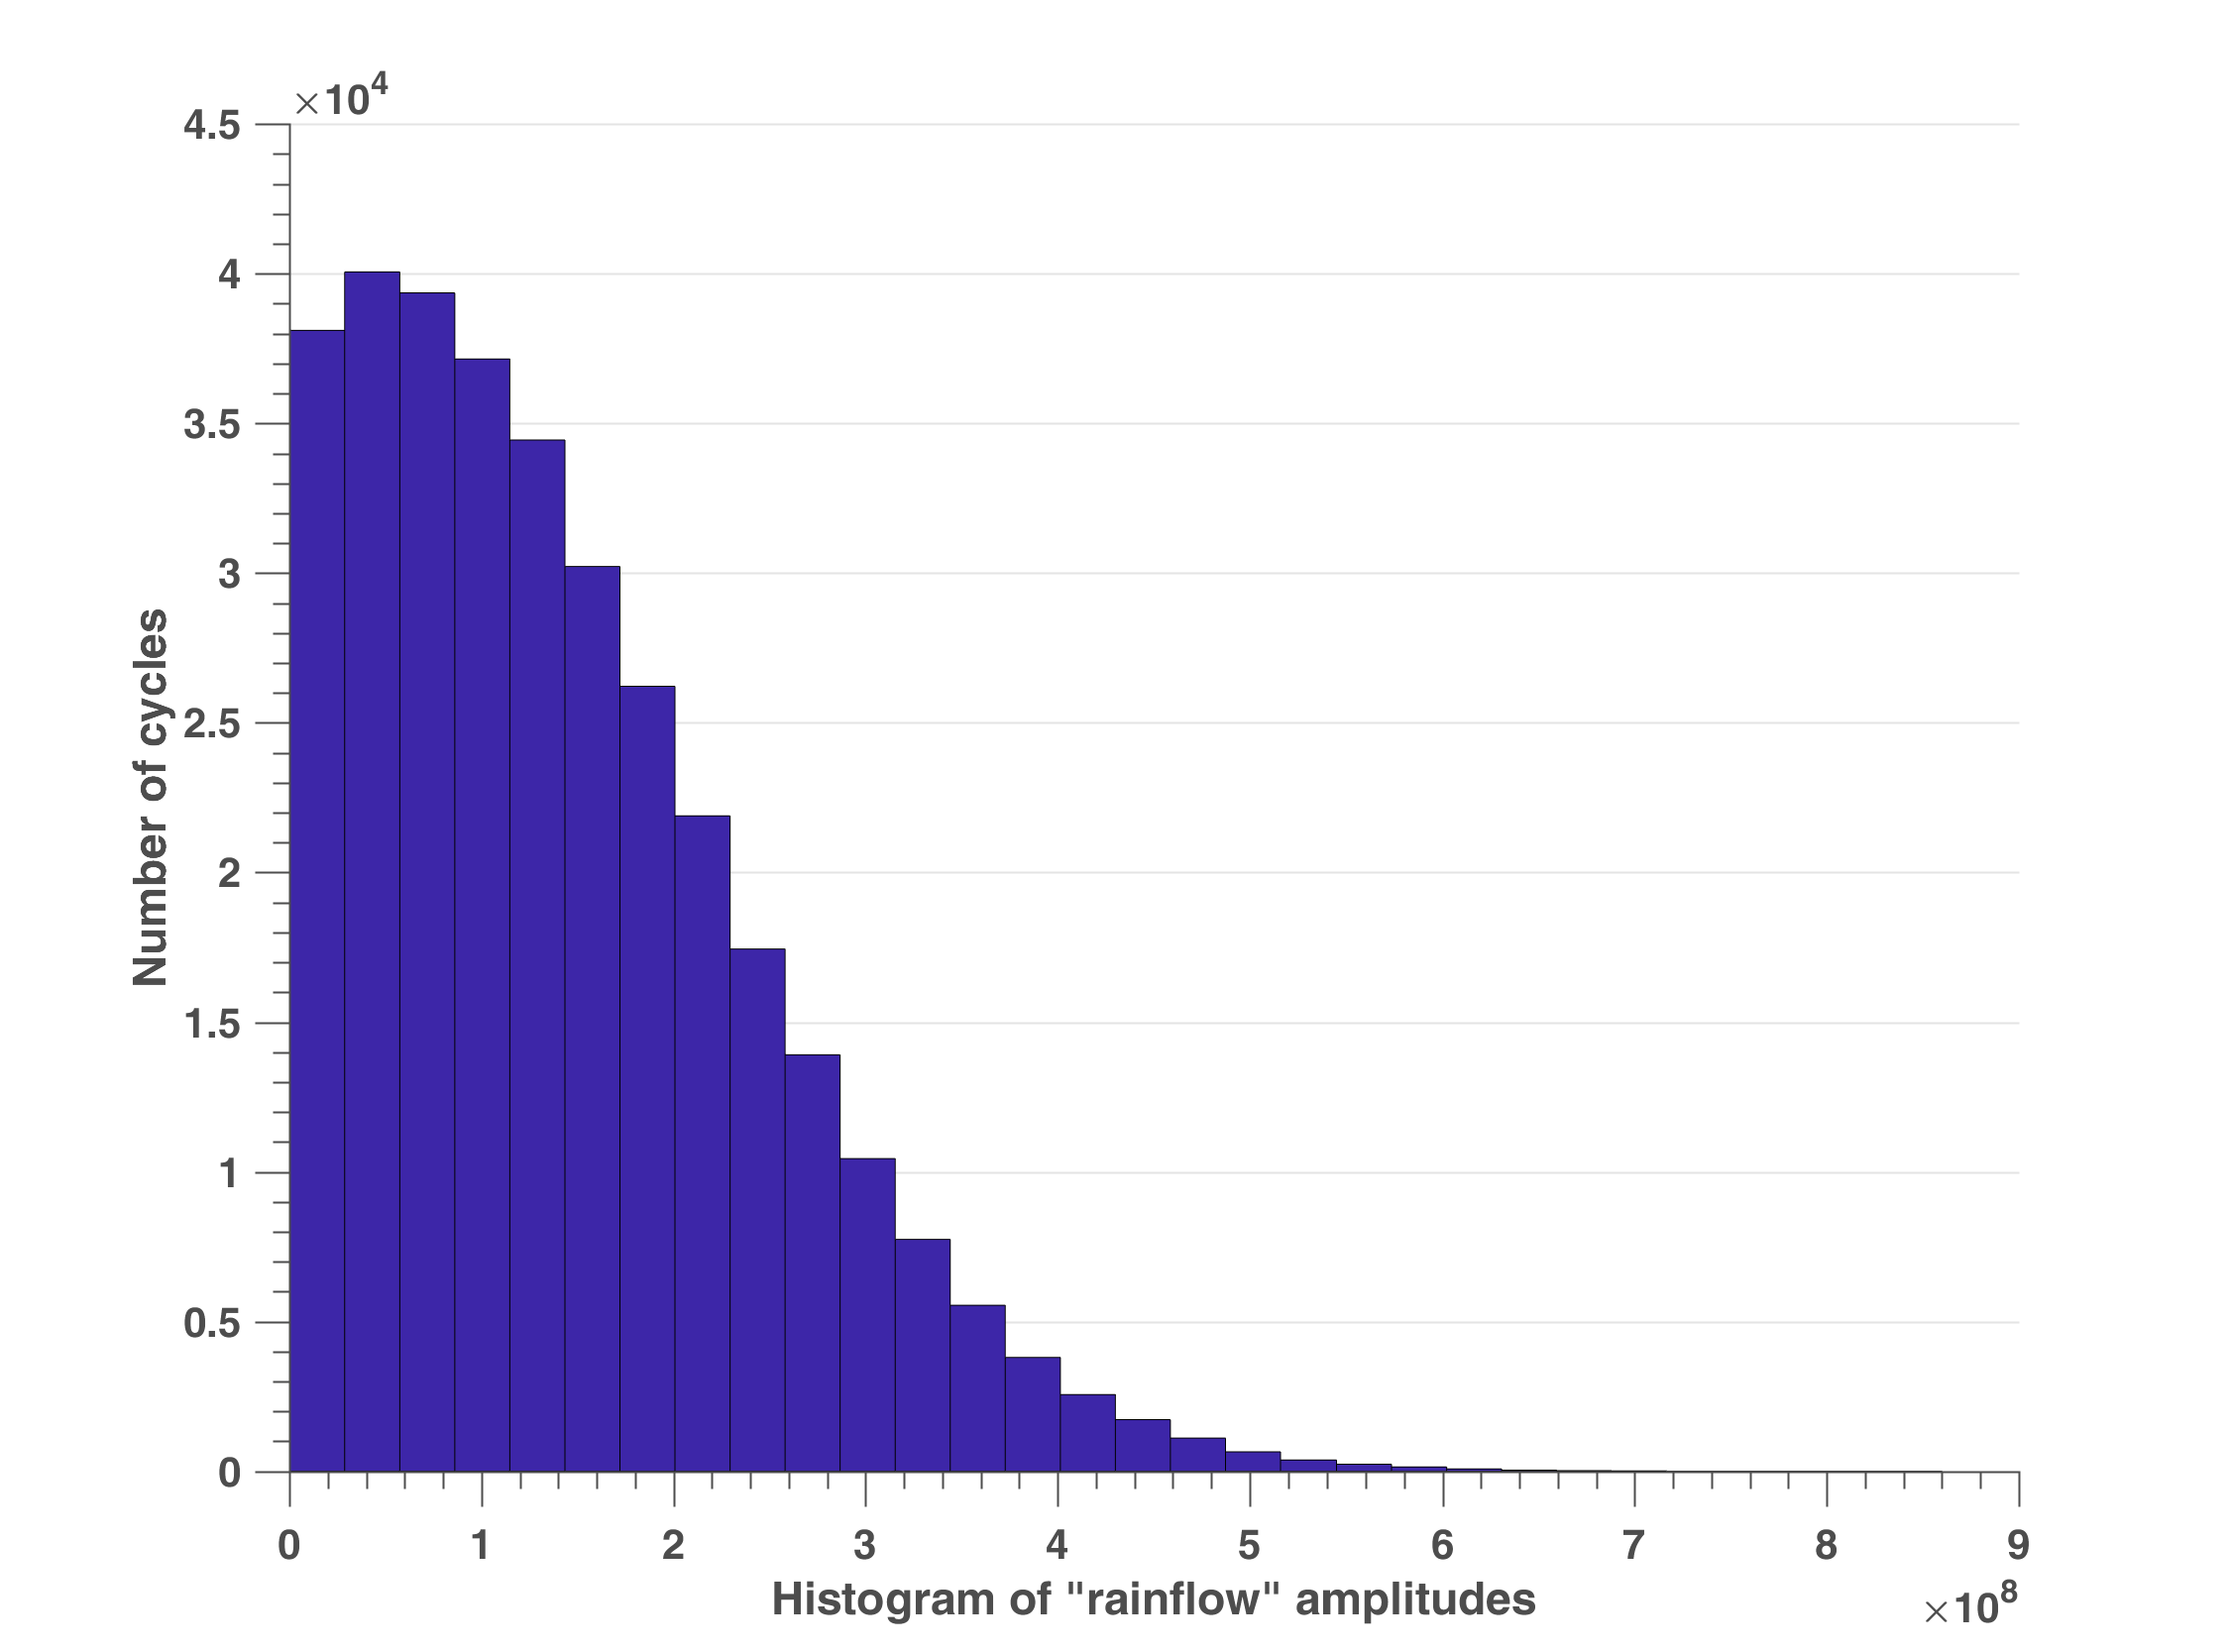
\includegraphics[width=\textwidth]{figures//randomdemo_ampl.png} 
	\caption{Amplitudes distribution extracted from \figref{randomdemo}}
	\label{randomdemoampl}
\end{figure}

\begin{figure}[!h]
	\centering
	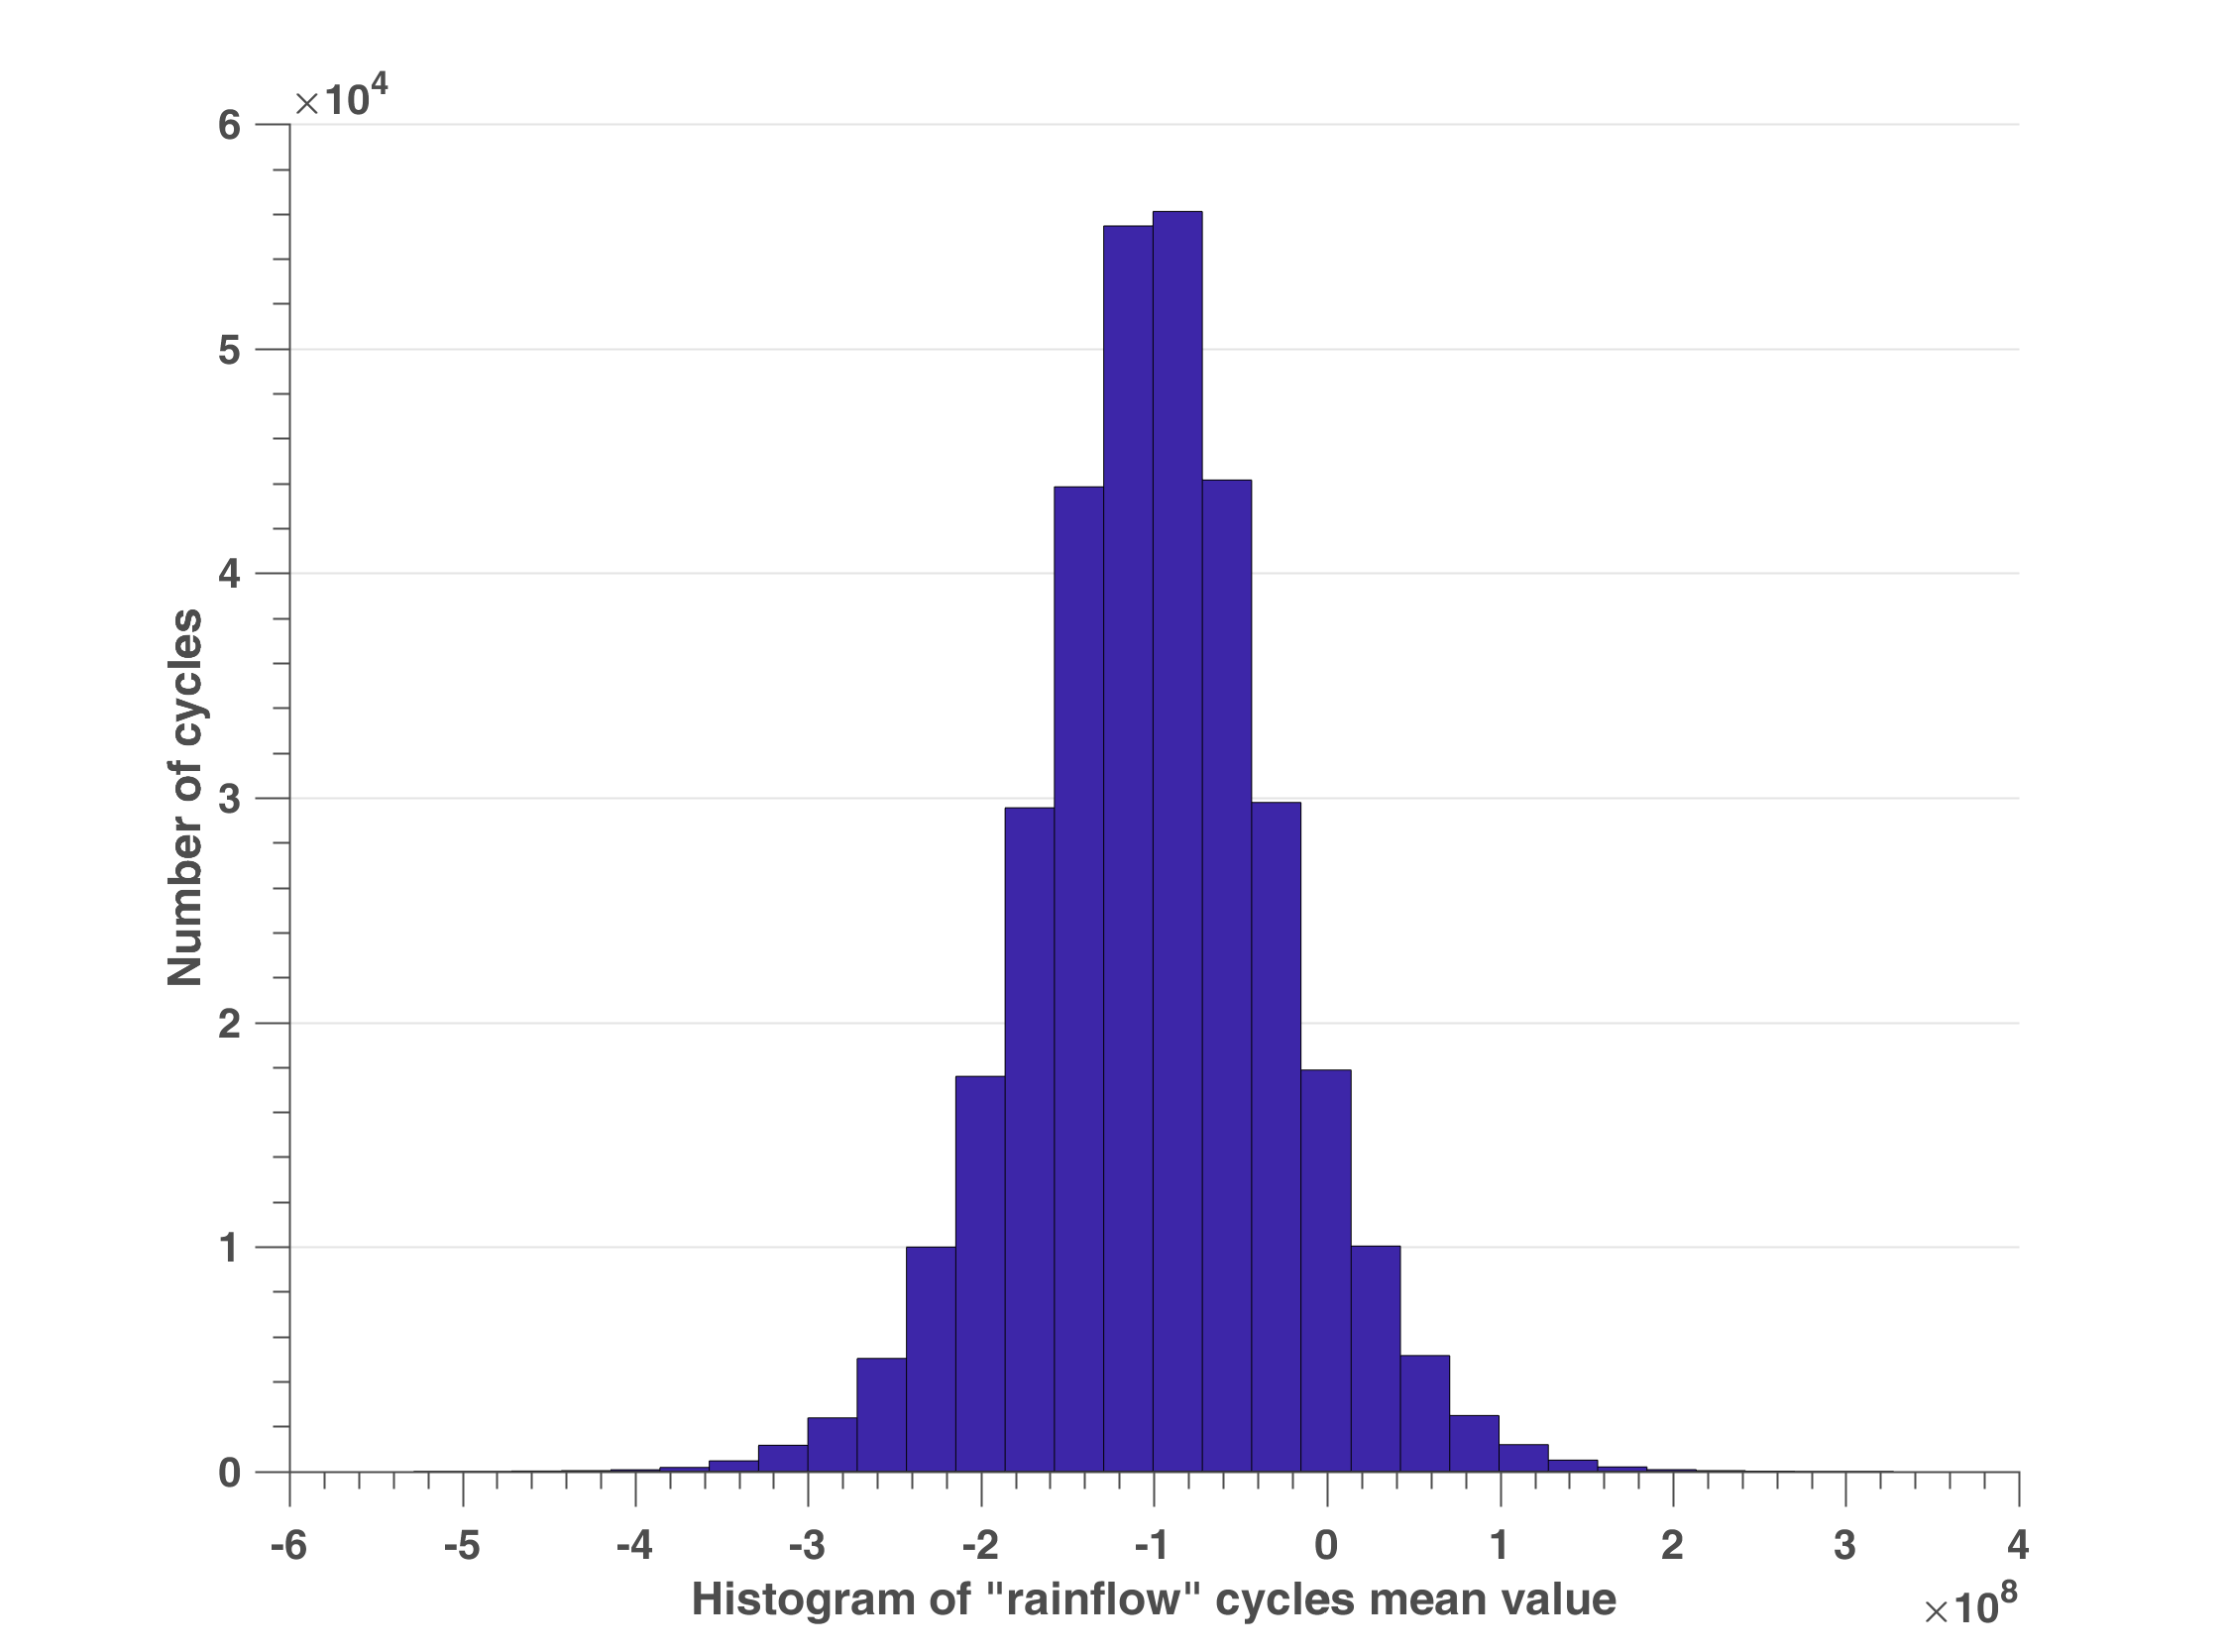
\includegraphics[width=\textwidth]{figures//randomdemo_mean.png} 
	\caption{Mean stresses distribution extracted from \figref{randomdemo}}
	\label{randomdemomean}
\end{figure}
\begin{figure}[!h]
	\centering
	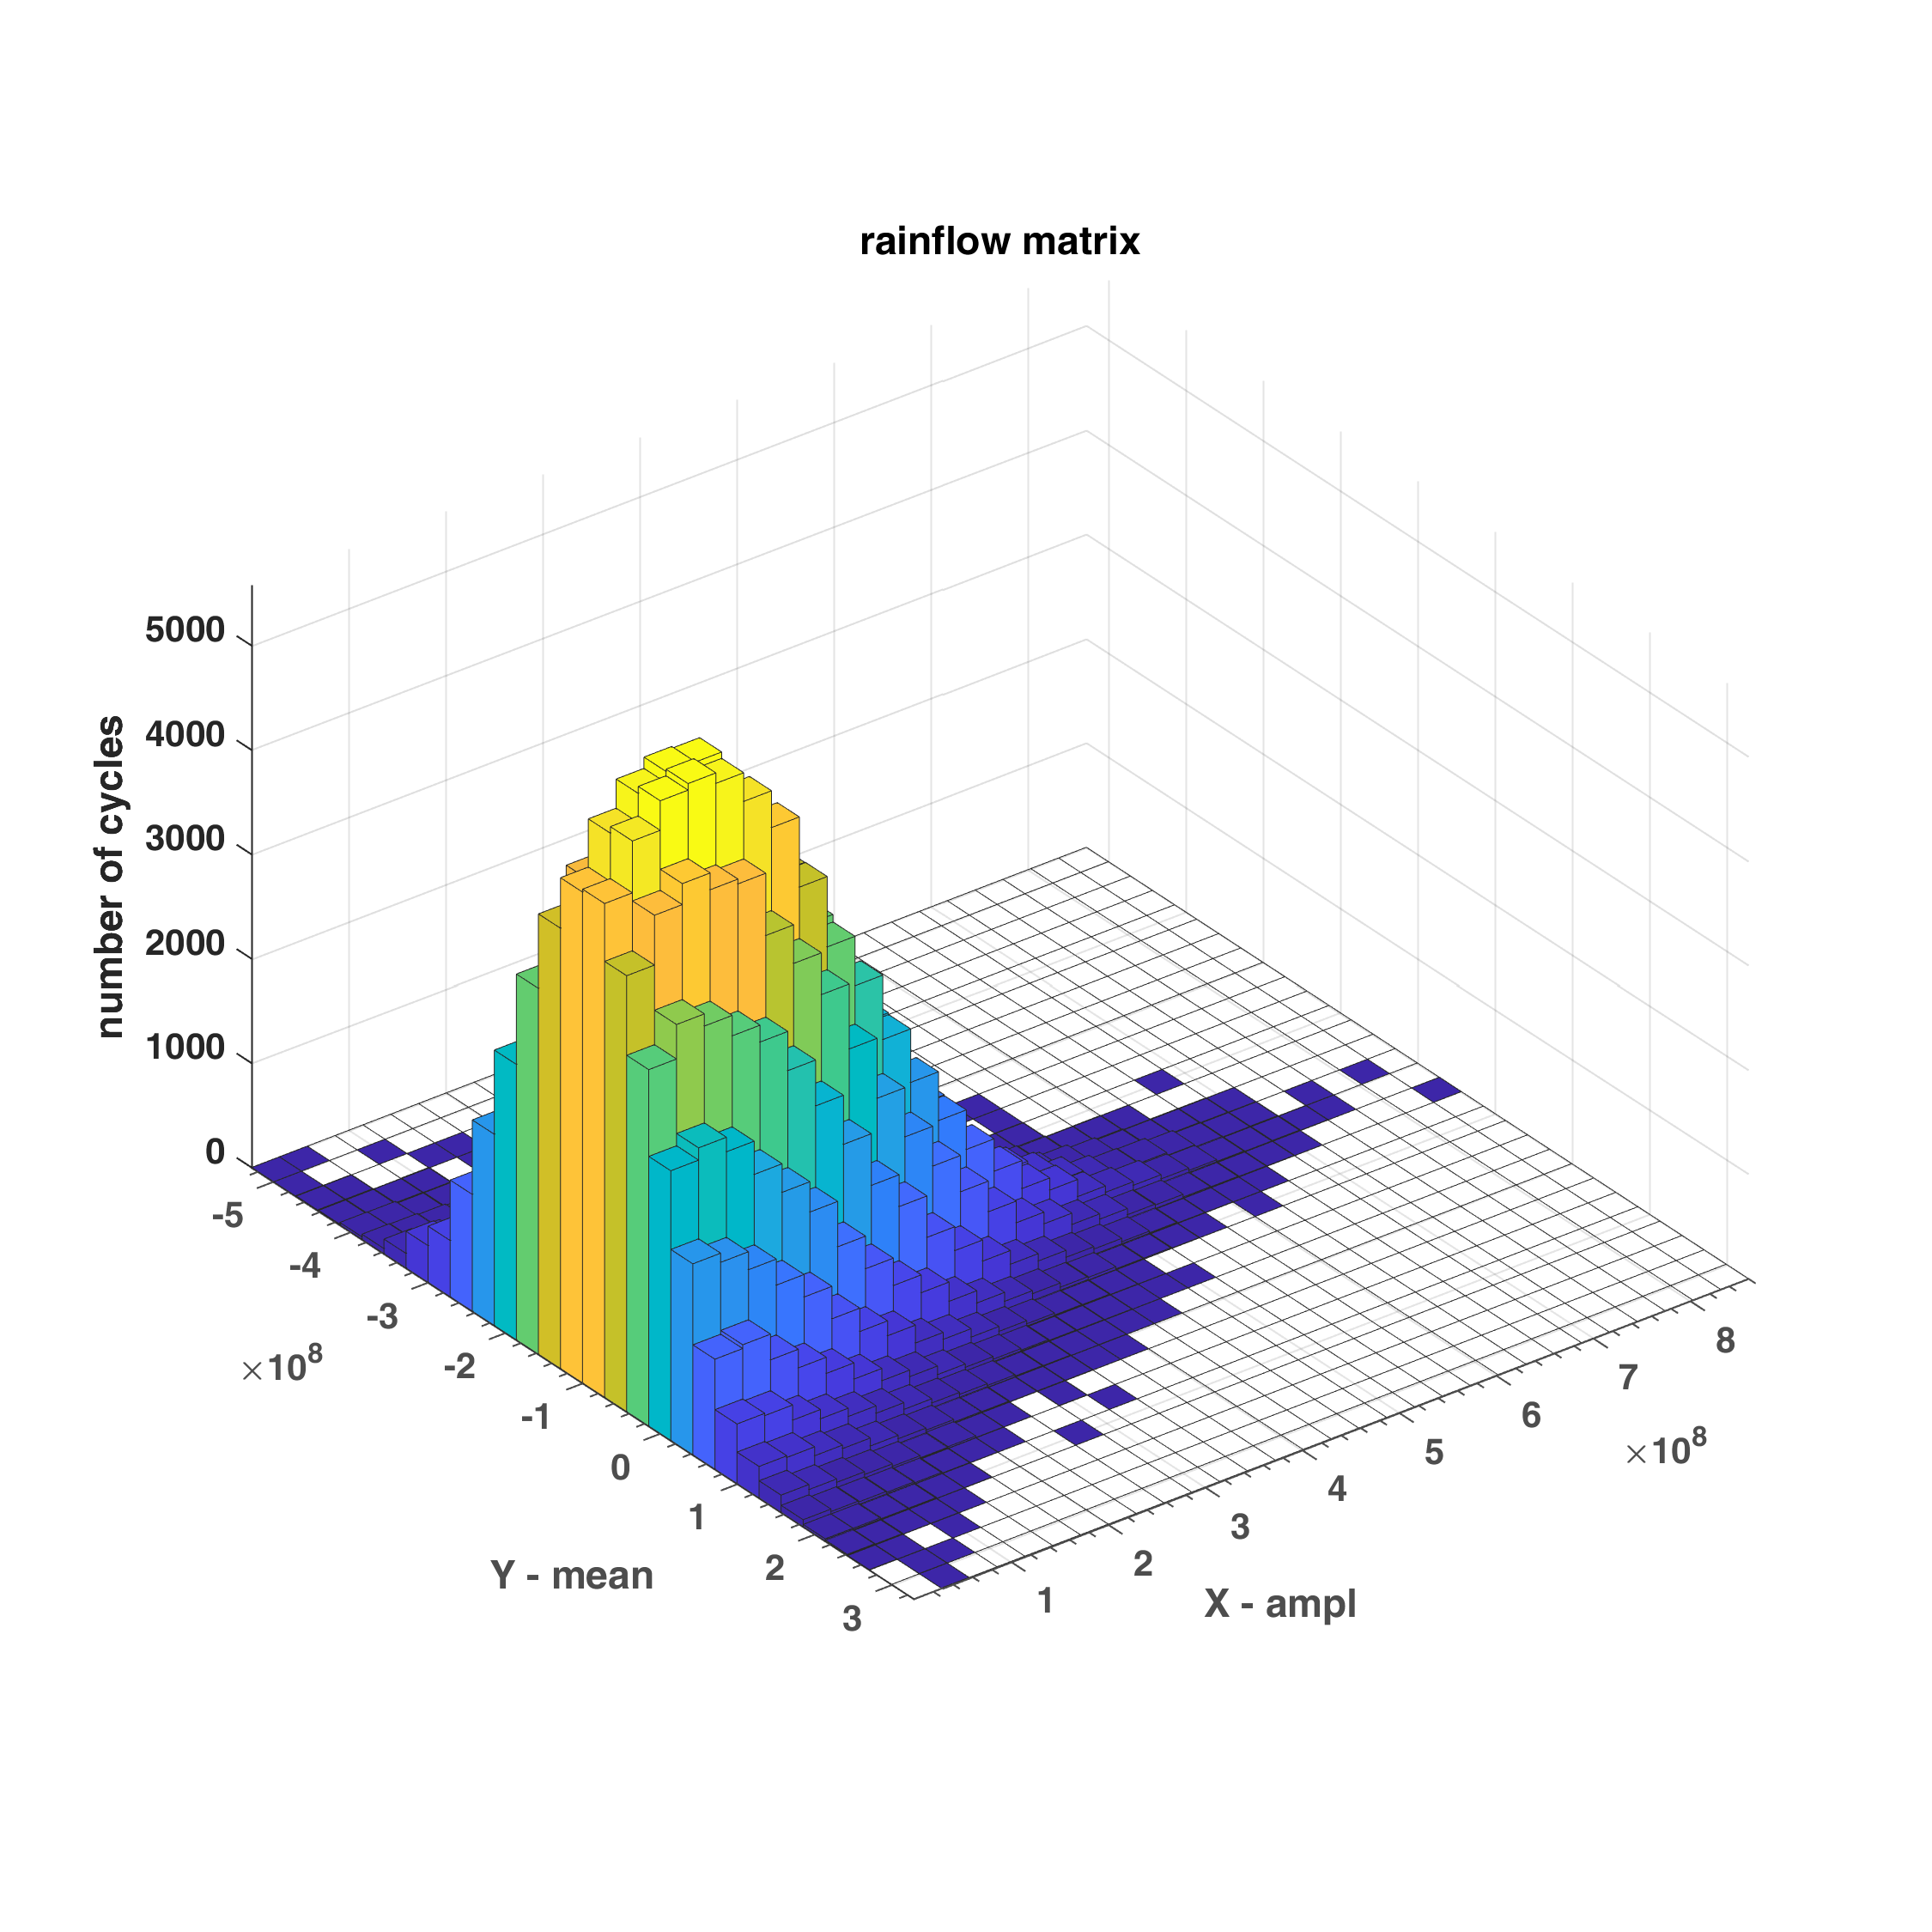
\includegraphics[width=\textwidth]{figures//randomdemo_3d.png} 
	\caption{Rainflow matrix extracted from \figref{randomdemo}}
	\label{randomdemo3d}
\end{figure}


